\documentclass [a4paper,12pt]{report}

\usepackage{geometry}
\geometry{a4paper,top=3cm,bottom=3cm,left=3cm,right=3cm,%
          heightrounded,bindingoffset=5mm}
\usepackage[T1]{fontenc}
\usepackage[utf8]{inputenc}
\usepackage[italian]{babel}
\usepackage[italian]{varioref}
\usepackage{braket}
\usepackage{graphicx}
\usepackage{amsmath}
\usepackage{fancyhdr}
\usepackage{amssymb}
\usepackage{caption}
\usepackage{rotating}
\usepackage{tabularx}
\usepackage{subcaption}
\usepackage{listings}
\usepackage{float}
\usepackage{hyperref}
\usepackage{xcolor} % Per utilizzare i colori personalizzati
\usepackage[utf8]{inputenc}


\captionsetup{tableposition=top,figureposition=bottom,font=small, format=hang,labelfont={sf,bf}}
\usepackage{float}
\usepackage{mathtools}
% \usepackage[autostyle,italian=guillemets,⟨altre opzioni⟩]{csquotes} \usepackage[⟨opzioni⟩,backend=biber]{biblatex}

\DeclarePairedDelimiter{\abs}{\lvert}{\rvert}
\DeclarePairedDelimiter{\norma}{\lVert}{\rVert}

\newcommand{\clearemptydoublepage}{\newpage{\pagestyle{empty}\cleardoublepage}}

\begin{document}

\pagestyle{fancy}

\renewcommand{\chaptermark}[1]{\markboth{#1}{}}
\renewcommand{\sectionmark}[1]{\markright{\thesection\ #1}}
\fancyhf{} \fancyhead[LE,RO]{\bfseries\thepage}
\fancyhead[LO]{\bfseries\rightmark}
\fancyhead[RE]{\bfseries\leftmark}
\renewcommand{\headrulewidth}{0.5pt}
\renewcommand{\footrulewidth}{0pt}
\fancypagestyle{plain}{
\fancyhead{}
\renewcommand{\headrulewidth}{0pt}}

\thispagestyle{empty}

%titolo
\begin{center}
    \large
    \textit{UNIVERSITÀ POLITECNICA DELLE MARCHE\\}
  %\normalsize
    \vspace*{.5cm}
  \textit{ FACOLTÀ DI INGEGNERIA \\}  
\end{center}

%immagine logo univpm
\begin{figure}[h]
    \centering
    
\includegraphics[width=5cm]{files/logo.png}
\end{figure}

%titolo tesi e corso di università
\begin{center}
%inserimento di distanza 0.5 cm
  \vspace*{0.5cm} 
  \emph{Corso di Laurea Magistrale in\\Ingegneria Informatica e dell'Automazione\\}
	\hfill \\
  \vspace*{.75cm} \large %true
  \emph{\textbf{HARDWARE-IN-THE-LOOP PX4 – MATLAB UAV TOOLBOX.}}
  \par
\noindent\rule{.3\textwidth}{1pt}\par\vspace{0.5cm}
\emph{\textbf{\textit{HARDWARE-IN-THE-LOOP PX4 – MATLAB UAV TOOLBOX}}}
\end{center}


%flushleft vuol dire testo allineato a sinistra
%textsc -> LETTERE MAIUSCOLE

\vspace{2cm}
\begin{flushleft}
Professore:\\\textsc{\textbf{Prof. Freddi Alessandro}}\\
\end{flushleft}
\vspace*{-1.55cm}
\begin{flushright}
Studente:\\\textsc{\textbf{Novelli Giovanni}}\\     
Studente:\\\textsc{\textbf{Cardoni Lorenzo}}\\ 
\end{flushright}
\vspace*{3.8cm}
%ANNO ACCADEMICO
\begin{center}
\large{\textsc{Anno Accademico 2023-2024}}
\end{center} \clearpage


%mi crea l'indice
\tableofcontents


%setta il tipo di contatore per l'indice
\setcounter{secnumdepth}{3}
\clearemptydoublepage
\chapter{Introduzione}
\section{UAV}
\begin{figure}[h]
    \centering
    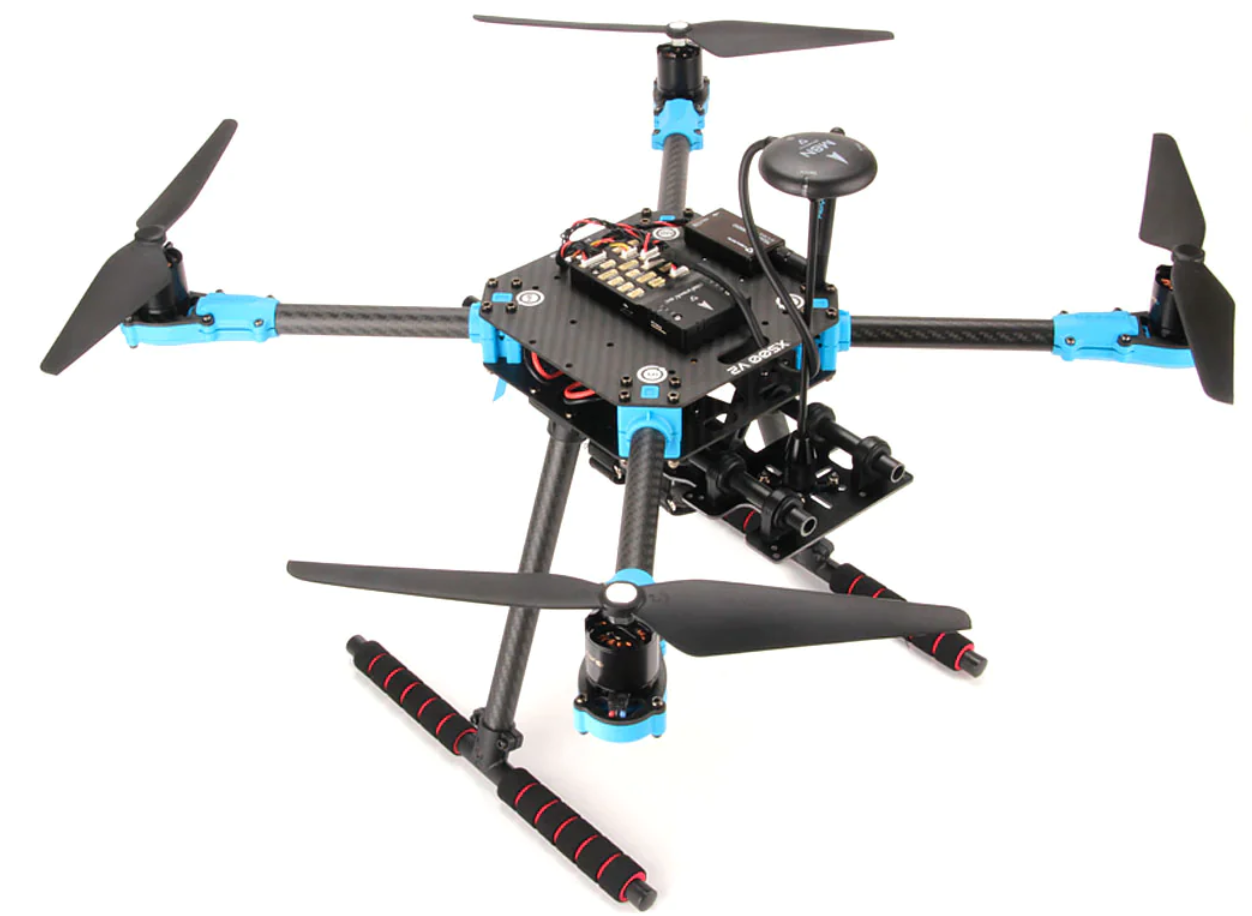
\includegraphics[width=0.7\linewidth]{files/drone.png}
    \caption{Quadricottero Holybro}
    \label{fig:enter-label}
\end{figure}
Un veicolo aereo senza equipaggio (UAV), noto anche come drone, è un aeromobile autonomo che opera senza la presenza umana a bordo. Attualmente, gli UAV sono ampiamente utilizzati in svariate applicazioni, tra cui la fotografia aerea, l'agricoltura di precisione, il monitoraggio ambientale, la sorveglianza e il trasporto.
\\~\\
Dal punto di vista tecnico, il controllo di un drone coinvolge diverse componenti hardware e software:
\subsubsection*{Hardware:}
\begin{itemize}
    \item \textbf{Microprocessore Primario:} Il cuore del sistema di controllo, responsabile dell'esecuzione delle istruzioni di volo.
    \item \textbf{Processore Secondario (Failsafe):} Garantisce la sicurezza del volo intervenendo in situazioni di emergenza o malfunzionamenti del sistema principale.
    \item \textbf{Attuatori:} Include regolatori di velocità elettronici (ESCs) che gestiscono la potenza fornita ai motori, controllando così il movimento del drone.
    \item \textbf{Sensori a Gradi di Libertà (DOF):} Per esempio, giroscopi e accelerometri a 3 assi (6DOF) per monitorare l'orientamento e il movimento del drone. Sensori a 11DOF possono includere barometro, bussola e GPS per una maggiore precisione.
\end{itemize}

\subsubsection*{Software:}
\begin{itemize}
    \item \textbf{Autopilota o Stack di Volo:} Responsabile dell'esecuzione delle missioni di volo in modo autonomo o in risposta a input remoti. Gestisce la stabilizzazione, il controllo degli attuatori e la navigazione.
    \item \textbf{Firmware:} Il software incorporato che gestisce il codice macchina, l'esecuzione del processore e l'accesso alla memoria. Deve essere altamente affidabile e efficiente.
    \item \textbf{Middleware:} Gestisce la comunicazione tra i vari componenti del sistema, facilitando il flusso di dati e comandi tra sensori, attuatori e autopilota.
    \item \textbf{Sistema Operativo:} Ad esempio, ROS (Robot Operating System), Nuttx o Linux, fornisce un ambiente operativo che consente di eseguire complesse operazioni di controllo, pianificazione di volo e acquisizione dati in tempo reale.
\end{itemize}
Gli UAV operano in tempo reale, richiedendo una rapida elaborazione dei dati sensoriali. L'integrazione efficiente tra hardware e software è essenziale per garantire il controllo stabile e sicuro del drone durante tutte le fasi della missione.
\\~\\
L'evoluzione dei sistemi integrati, come i veicoli senza pilota, con unità di controllo e vari sensori complessi, ha reso i tradizionali test su macchine reali costosi e complessi, data la presenza di molteplici sensori come IMU, georadar e termocamere. L'impiego del concetto "Hardware-In-The-Loop" (HITL) emerge come soluzione strategica. Questa metodologia consente di condurre test completi senza la necessità di utilizzare direttamente sul campo un prodotto finale assemblato, affrontando la sfida delle grandi mole di dati e riducendo i costi associati ai test in tempo e spazio reali.
\section{Hardware-In-The-Loop (HITL)}
Il termine "Hardware-In-The-Loop" (HITL) si riferisce a una serie di metodologie utilizzate per verificare il funzionamento di dispositivi hardware connessi a una piattaforma di simulazione in grado di emulare il comportamento del sistema reale. Questo approccio consente di testare gli algoritmi di controllo durante la fase di progettazione, eliminando la necessità di attendere la disponibilità del prodotto finale e riducendo tempi e costi associati ai test fisici.
\\~\\
Grazie all'utilizzo dell'HITL è possibile:
\begin{itemize}
    \item Creare e simulare una rappresentazione virtuale dei componenti fisici;
    \item Eseguire algoritmi di controllo sulla simulazione, permettendo l'interazione con il dispositivo fisico attraverso canali di Input/Output.
\end{itemize}
Questa metodologia risulta particolarmente vantaggiosa in situazioni in cui testare l'algoritmo di controllo direttamente sul sistema fisico sarebbe costoso e/o pericoloso. 
\section{Obiettivo del Progetto}
Il progetto mira a stabilire una connessione Hardware-In-The-Loop (HITL) tra PX4 ed il MATLAB UAV Toolbox, sfruttando le librerie disponibili per:
\begin{itemize}
    \item Log dei segnali del Flight Controller e del Plant Model
    \item Simulazione di guasti alle componenti di attuazione e sensoristica
    \item Sviluppo di algoritmi di rilevamento guasti
\end{itemize}
L'accesso alle misure sensoriali, combinato con la capacità di simulare guasti, fornisce la base per lo sviluppo di algoritmi di diagnosi o di controllo tollerante ai guasti.
\\~\\
Il percorso del progetto prevede le seguenti fasi indicative:
\begin{itemize}
    \item Installazione e configurazione del software di simulazione con il modello del drone.
    \item Analisi del simulatore per identificare e comprendere le librerie disponibili.
    \item Implementazione della connessione HITL tra PX4 e MATLAB.
    \item Simulazione di un guasto e acquisizione dei dati sensoriali.
    \item Valutazione delle modalità per modificare il Flight Controller
    \item Sviluppare algoritmi di rilevamento guasti attraverso l'integrazione con il MATLAB UAV Toolbox.
\end{itemize}
L'obiettivo finale è ottenere una piattaforma funzionale che consenta di esplorare e implementare algoritmi avanzati di controllo e diagnostica per droni, migliorando la comprensione e la gestione dei guasti in un contesto di volo. \clearemptydoublepage
\chapter{Requisiti Progetto}
\section{Archittetura PX4}
PX4 rappresenta un software open source specializzato nel controllo di veicoli unmanned, offrendo ai programmatori una vasta gamma di strumenti e un supporto completo sia a livello software che hardware. Nella figura \ref{fig:PX4_Arch}, si presenta un quadro panoramico ad alto livello del controllore di volo implementato in PX4:
\begin{figure}[h]
    \centering
    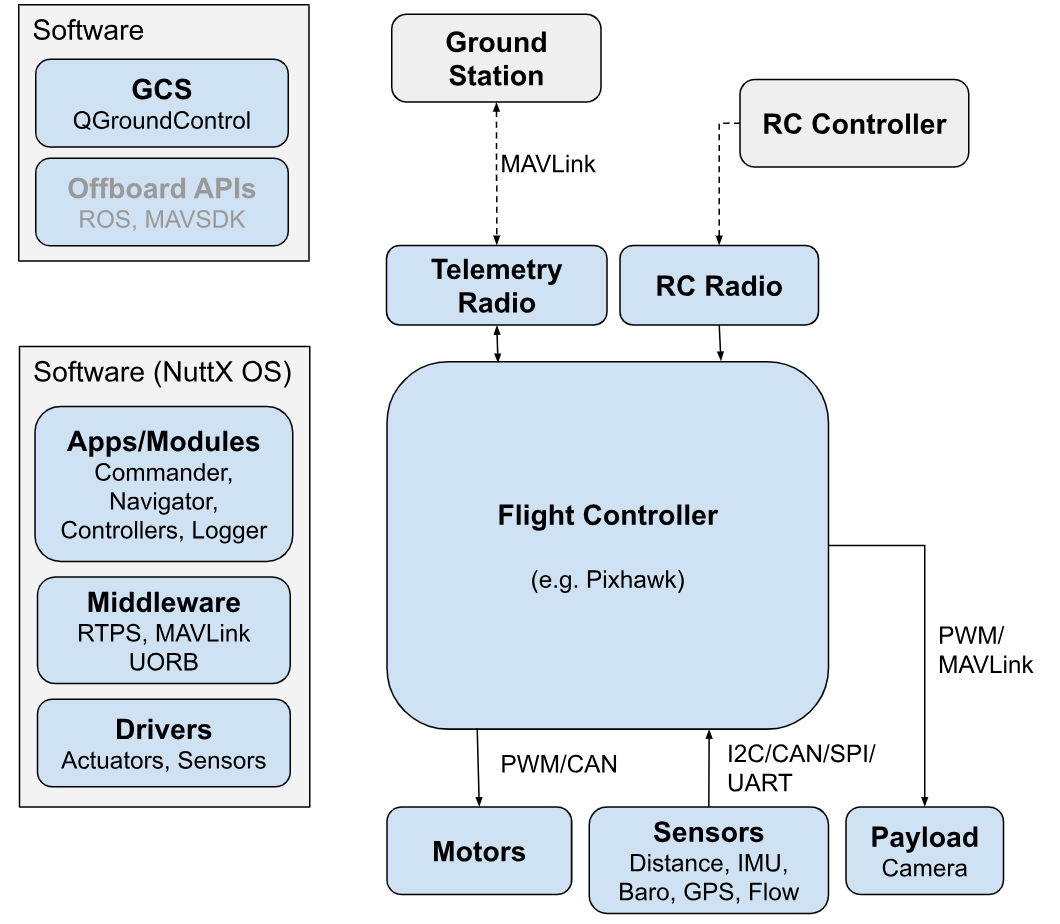
\includegraphics[width=0.7\linewidth]{PX4_Architettura.png}
    \caption{Architettura di alto livello del controllore di volo in PX4}
    \label{fig:PX4_Arch}
\end{figure}
\\
Dal lato hardware, la configurazione comprende diversi componenti chiave:
\begin{itemize}
    \item Controllore di volo (PixHawk): Esegue lo stack PX4, fornendo un'interfaccia fondamentale per la gestione complessiva del drone.
    \item ESC (Electronic Speed Control): Questi circuiti regolano la velocità e la direzione di rotazione dei motori, collegandosi alle uscite PWM del controller.
    \item Sensori: Connessi al controller tramite bus I2C o UART, forniscono dati essenziali per la navigazione e il controllo.
    \item Fotocamera: Collegata tramite canale PWM o protocollo MAVLink, consente la raccolta di dati visivi e può essere integrata nelle attività di controllo del drone.
    \item RC Controller: Necessario per il controllo manuale remoto attraverso un Joypad.
\end{itemize}
Sul fronte software, la configurazione include:
\begin{itemize}
    \item QGroundControl: Utilizzato come stazione di controllo da un computer host, fornisce un'interfaccia utente per monitorare e comandare il drone.
    \item Stack di volo PX4: Eseguito sul controllore di volo, comprende moduli di comunicazione, driver e middleware. La sua architettura di alto livello è rappresentata nella Figura 
\end{itemize}

 \clearemptydoublepage
\chapter{Configurazione dell'Ambiente di Sviluppo in Simulink per il Sistema PX4 Hardware-in-the-Loop (HITL)}
Per configurare il firmware PX4 per la simulazione Hardware-in-the-Loop (HITL), è necessario seguire i seguenti passaggi

\section{Configurazione QGroundControl}

Nella schermata di download di QGroundControl per la configurazione hardware, scarica e installa QGC.
Dopo l'installazione, clicca su "Verify Installation" per verificare che l'installazione sia avvenuta correttamente.
Successivamente, clicca su "Next" per procedere.
\\
Seguire questi passaggi per configurare e impostare QGroundControl (QGC):
\begin{itemize}
    \item Collegare l'autopilot a QGC tramite USB.
    \item Abilitare la modalità HITL.
    \item Navigare fino alla sezione Setup > Safety.
    \item Selezionare Enabled dalla lista HITL Enabled.
    \item Selezionare il telaio (Airframe).
    \item Navigare fino a Setup > Airframes.
    \item Selezionare HIL QuadCopter per simulare un quadricottero. Fare clic su Apply and Restart nella parte superiore destra della pagina di configurazione del telaio.
    \item Nella scheda Generale del menu delle impostazioni, deselezionare tutte le opzioni di AutoConnect tranne UDP.
    \\
    \textbf{Nota}: Questa selezione interrompe la comunicazione tra QGC e l'autopilot PX4 tramite USB. QGC può ora comunicare solo tramite UDP (di solito gestito da un Simulatore che funge da ponte tra QGC e l'autopilot e collega i dati MAVLink tra QGC e l'autopilota tramite UDP).
    \\
    \item Chiudere QGC.
\end{itemize}
\noindent

Continua con i passaggi successivi nel processo di configurazione hardware per la costruzione del firmware. 
\\
Assicurati di verificare che la compilazione sia avvenuta con successo.

\section{Configurazione del Modello del Controller PX4 in Simulink}
Eseguire questi passaggi per configurare il modello Simulink.

Nella scheda Modeling, fare clic su Model Settings.

Nella finestra di dialogo Configuration Parameters, selezionare PX4 Pixhawk 6x (Fig. \ref{fig:Hardware Board}).
\begin{figure}[H] % Opzione [h] posiziona la figura qui (here)
  \centering
  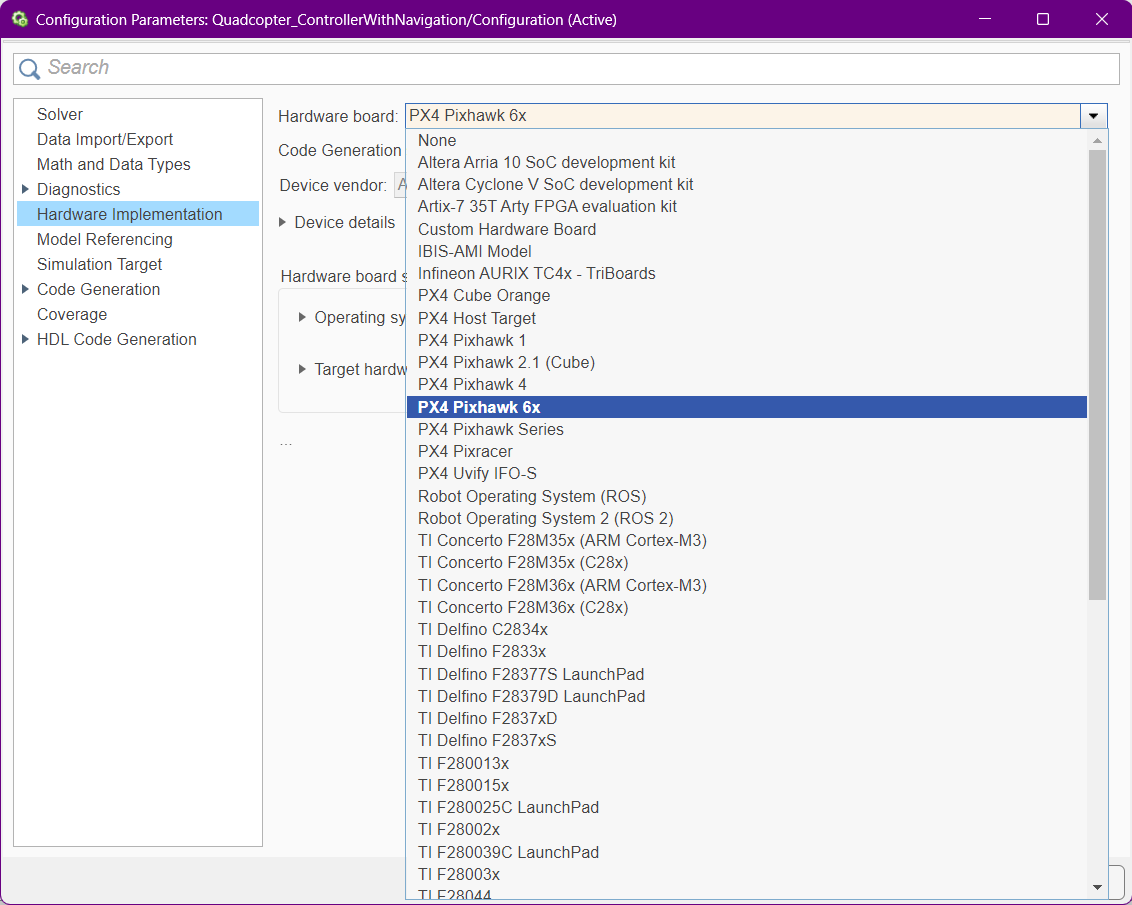
\includegraphics[width=0.8\textwidth]{files/images/matlab1.png} % Imposta la larghezza dell'immagine al 50% della larghezza del testo
  \caption{Hardware Board} % Didascalia sotto l'immagine
  \label{fig:Hardware Board} % Etichetta per fare riferimento all'immagine nel testo
\end{figure}
\noindent
Fare clic su HITL e quindi selezionare Enable HITL Mode (Fig. \ref{fig:HITL}).
\begin{figure}[H] % Opzione [h] posiziona la figura qui (here)
  \centering
  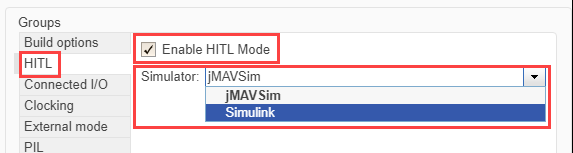
\includegraphics[width=0.8\textwidth]{files/images/HITL.png} % Imposta la larghezza dell'immagine al 50% della larghezza del testo
  \caption{HITL} % Didascalia sotto l'immagine
  \label{fig:HITL} % Etichetta per fare riferimento all'immagine nel testo
\end{figure}
\noindent
Selezionare il simulatore da eseguire per HITL.
\\
Fare clic su MAVLink e assicurarsi che l'opzione Enable MAVLink su /dev/ttyACM0 sia selezionata (Fig. \ref{fig:MAVLink}).
\begin{figure}[H] % Opzione [h] posiziona la figura qui (here)
  \centering
  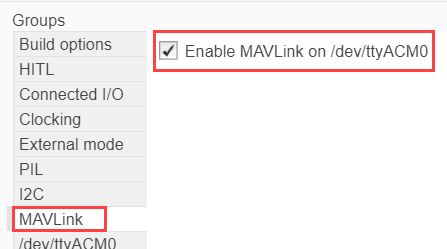
\includegraphics[width=0.8\textwidth]{files/images/MAVLink.png} % Imposta la larghezza dell'immagine al 50% della larghezza del testo
  \caption{MAVLink} % Didascalia sotto l'immagine
  \label{fig:MAVLink} % Etichetta per fare riferimento all'immagine nel testo
\end{figure}
\noindent
Fare clic su Apply e quindi su OK.


\section{Configurazione del Toolchain Cygwin e Download del Codice Sorgente PX4}
Questa sezione spiega il compito da completare come parte del passo "Configurazione del Toolchain Cygwin e Download del Codice Sorgente" del processo di configurazione hardware (utilizzando le schermate di configurazione hardware). 
\\
\textbf{Nota}: Assicurati che il tuo PC sia connesso a una connessione internet attiva prima di procedere con questo passaggio.
Per configurare il toolchain Cygwin™ e scaricare il codice sorgente PX4® utilizzato nel pacchetto di supporto per PX4 Autopilots nel UAV Toolbox, seguire questi passaggi:
\\
Scaricare la versione 0.8 di PX4 Cygwin Toolchain MSI Installer (Fig. \ref{fig:Download PX4 Cygwin Toolchain MSI Installer}), che è compatibile con PX4 Firmware v1.12.3, disponibile a questo \href{https://github.com/PX4/PX4-windows-toolchain/releases/tag/v0.8}{\textcolor{blue}{link}}.

\begin{figure}[H] % Opzione [h] posiziona la figura qui (here)
  \centering
  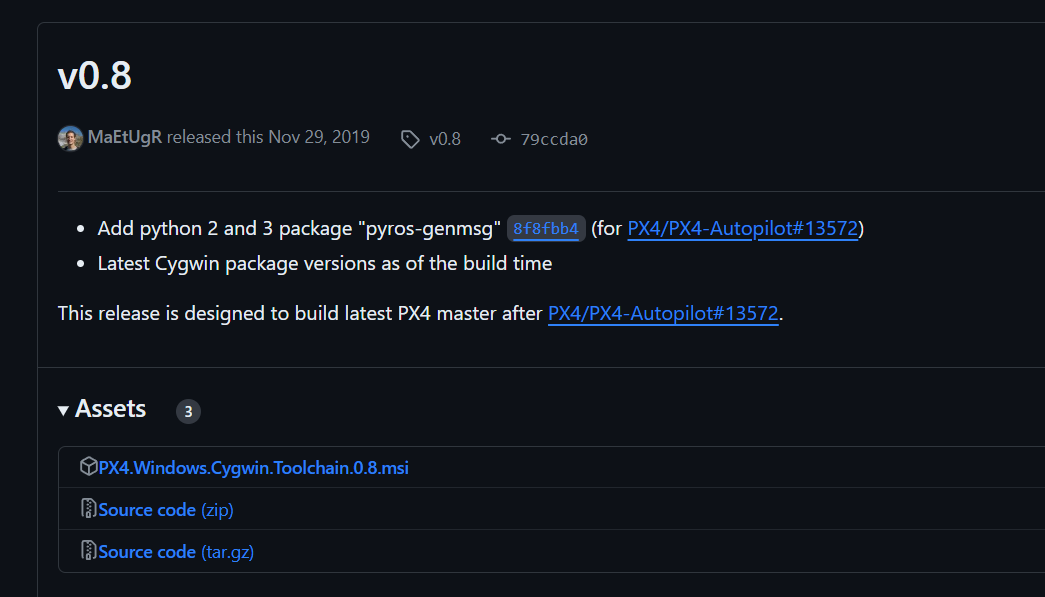
\includegraphics[width=0.8\textwidth]{files/images/github_cywing.png} % Imposta la larghezza dell'immagine al 50% della larghezza del testo
  \caption{Download PX4 Cygwin Toolchain MSI Installer} % Didascalia sotto l'immagine
  \label{fig:Download PX4 Cygwin Toolchain MSI Installer} % Etichetta per fare riferimento all'immagine nel testo
\end{figure}
\noindent
Nota: Il pacchetto di supporto UAV Toolbox per PX4 Autopilots supporta solo la versione v0.8 di PX4 Windows® Cygwin Toolchain MSI Installer, anche se una versione più recente potrebbe essere disponibile.
\\
Eseguire il programma di installazione MSI e avviare l'installazione del toolchain (Fig. \ref{fig:PX4 Toolchain Setup}).
\begin{figure}[H] % Opzione [h] posiziona la figura qui (here)
  \centering
  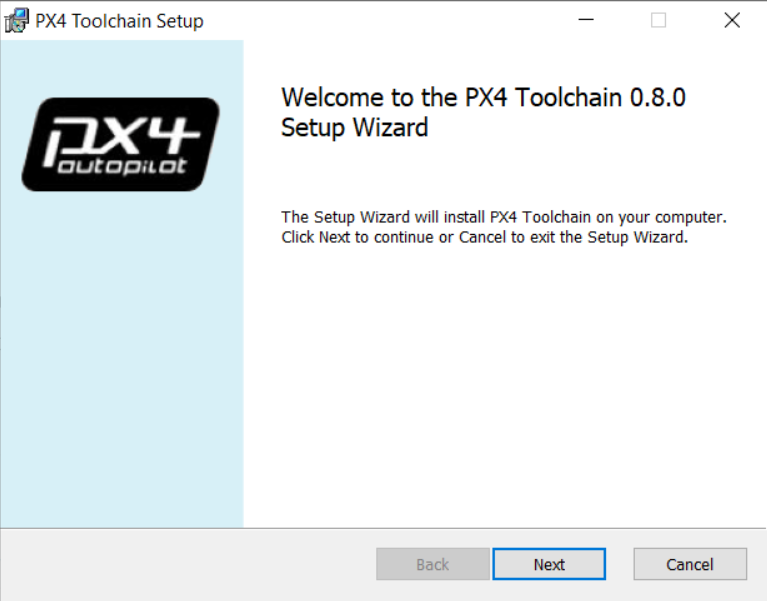
\includegraphics[width=0.8\textwidth]{files/images/setup_toolchain.png} % Imposta la larghezza dell'immagine al 50% della larghezza del testo
  \caption{PX4 Toolchain Setup} % Didascalia sotto l'immagine
  \label{fig:PX4 Toolchain Setup} % Etichetta per fare riferimento all'immagine nel testo
\end{figure}
\noindent
Cambiare la cartella di installazione per Cygwin in una qualsiasi cartella locale (ad esempio, C:\textbackslash{}px4), quindi fare clic su OK (Fig. \ref{fig:Selezione della cartella di installazione}).
\begin{figure}[H] % Opzione [h] posiziona la figura qui (here)
  \centering
  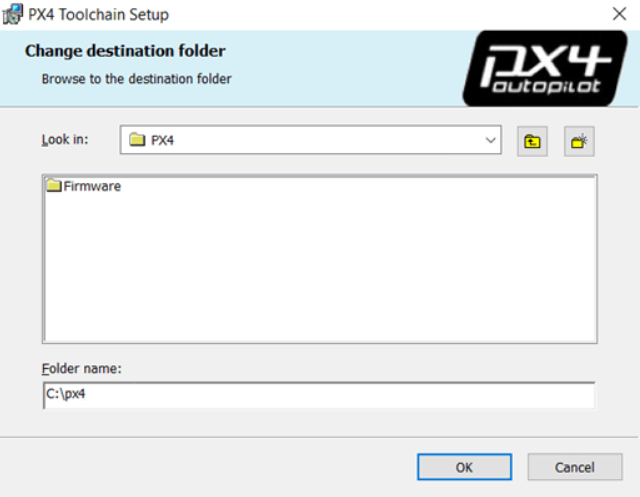
\includegraphics[width=0.8\textwidth]{files/images/folder_name.png} % Imposta la larghezza dell'immagine al 50% della larghezza del testo
  \caption{Selezione della cartella di installazione} % Didascalia sotto l'immagine
  \label{fig:Selezione della cartella di installazione} % Etichetta per fare riferimento all'immagine nel testo
\end{figure}
\noindent
All'ultimo passaggio della procedura guidata di configurazione del toolchain PX4, fare quanto segue:
\begin{itemize}
    \item Se non si dispone del Codice Sorgente PX4 (Firmware Autopilota PX4 v1.12.3) scaricato nel computer host, selezionare l'opzione "Clona repository PX4 e Avvia Simulazione", quindi fare clic su Fine. Questa opzione clona il firmware PX4 attuale. Quando si fa clic su Verifica Installazione nel passaggio 6 di seguito, il firmware viene automaticamente controllato alla versione v1.12.3.
    \item Se il Codice Sorgente PX4 (Firmware Autopilota PX4 v1.12.3) è già disponibile nel computer host, fare clic su Fine senza selezionare l'opzione "Clona repository PX4 e Avvia Simulazione" (Fig. \ref{fig:Clona repository PX4 e Avvia Simulazione}).
\end{itemize}
\begin{figure}[H] % Opzione [h] posiziona la figura qui (here)
  \centering
  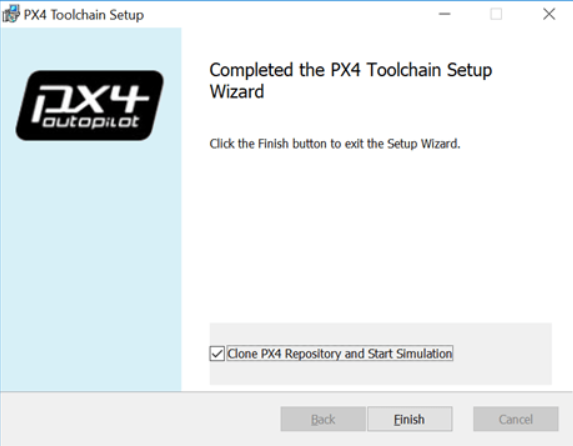
\includegraphics[width=0.8\textwidth]{files/images/clone_px4.png} % Imposta la larghezza dell'immagine al 50% della larghezza del testo
  \caption{Clona repository PX4 e Avvia Simulazione} % Didascalia sotto l'immagine
  \label{fig:Clona repository PX4 e Avvia Simulazione} % Etichetta per fare riferimento all'immagine nel testo
\end{figure}
\noindent
Se si è selezionata l'opzione "Clona repository PX4 e Avvia Simulazione" e si è fatto clic su Fine, viene avviata una shell bash che avvia la clonazione del firmware (Fig. \ref{fig:Shell bash che avvia la clonazione del firmware}).
\begin{figure}[H] % Opzione [h] posiziona la figura qui (here)
  \centering
  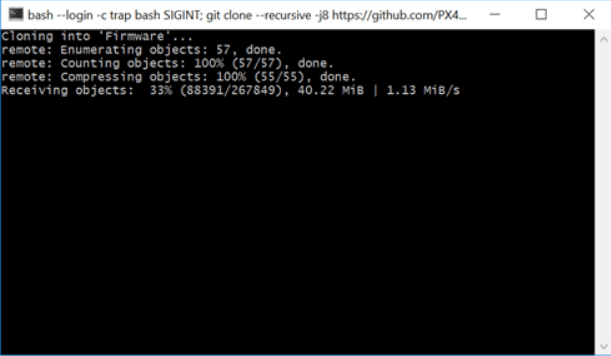
\includegraphics[width=0.8\textwidth]{files/images/bash_after_installation.png} % Imposta la larghezza dell'immagine al 50% della larghezza del testo
  \caption{Shell bash che avvia la clonazione del firmware} % Didascalia sotto l'immagine
  \label{fig:Shell bash che avvia la clonazione del firmware} % Etichetta per fare riferimento all'immagine nel testo
\end{figure}
\noindent
Attendere il completamento della clonazione del firmware. Dopo che il firmware è stato clonato, la Simulazione viene avviata in jMAVSim. È possibile chiudere la shell bash in questa fase.
\\
Il firmware PX4 viene clonato all'interno di una cartella denominata home, all'interno della cartella Cygwin selezionata durante l'installazione (ad esempio, C:\textbackslash{}px4\textbackslash{}home).

\section{Configurazione Firmware PX4 per l'Hardware-in-the-Loop}
Seguendo questi passaggi, il firmware PX4 sarà configurato correttamente per la simulazione Hardware-in-the-Loop (HITL) utilizzando il supporto per PX4 Autopilots nel UAV Toolbox. Questo ti permetterà di eseguire la simulazione HITL e verificare gli algoritmi di controllo implementati.
\\
Selezione del Firmware PX4 e del Hardware di Destinazione:
\\
Accedi alla schermata di selezione del firmware PX4 e del hardware di destinazione nel UAV Toolbox Support Package for PX4 Autopilots. Clicca su "Manage" (Fig. \ref{fig:UAV Toolbox Support Package for PX4 Autopilots}) e successivamente su "setup" (Fig. \ref{fig:Manage Toolbox}).

\begin{figure}[htbp]
    \begin{minipage}[b]{0.5\linewidth} % Definisci la larghezza della prima minipage (50% della larghezza della pagina)
        \centering
        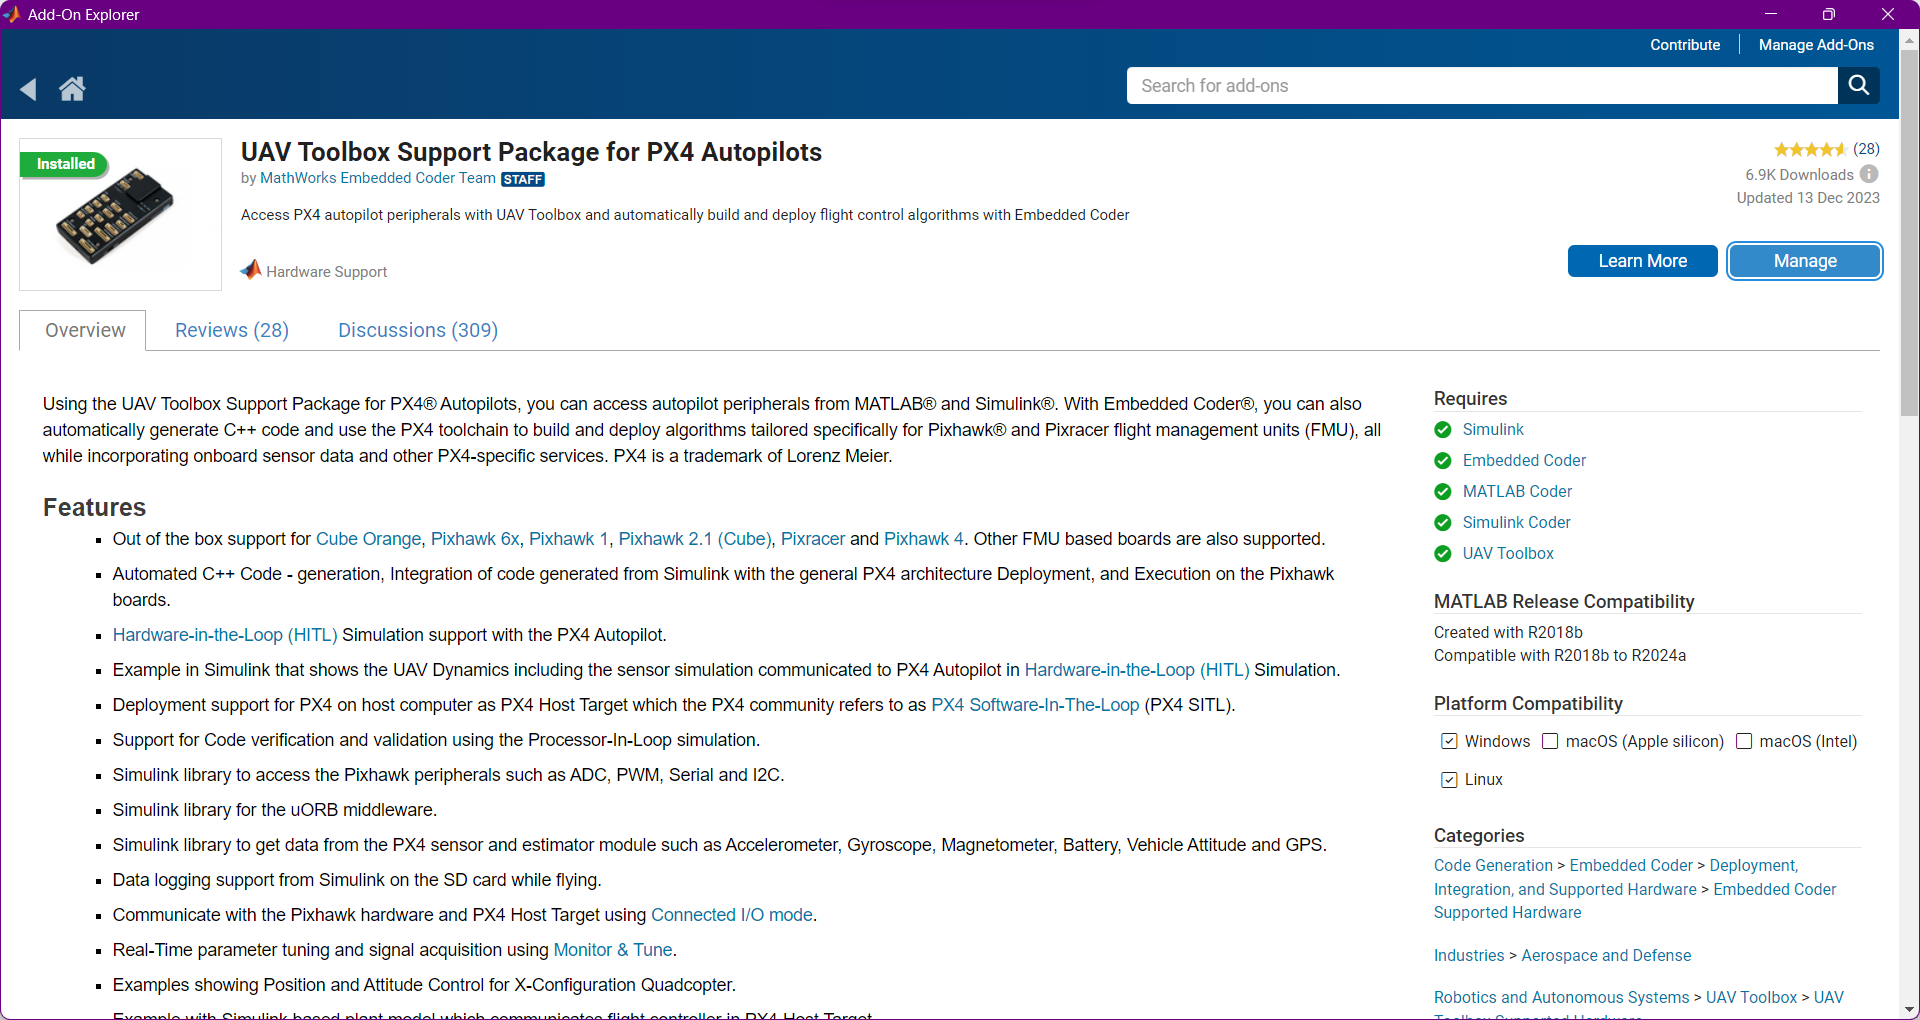
\includegraphics[width=\linewidth]{files/images/Screenshot 2024-03-13 120711.png} % Inserisci la prima immagine
        \caption{UAV Toolbox Support Package for PX4 Autopilots}
        \label{fig:UAV Toolbox Support Package for PX4 Autopilots}
    \end{minipage}%
    \begin{minipage}[b]{0.5\linewidth} % Definisci la larghezza della seconda minipage (50% della larghezza della pagina)
        \centering
        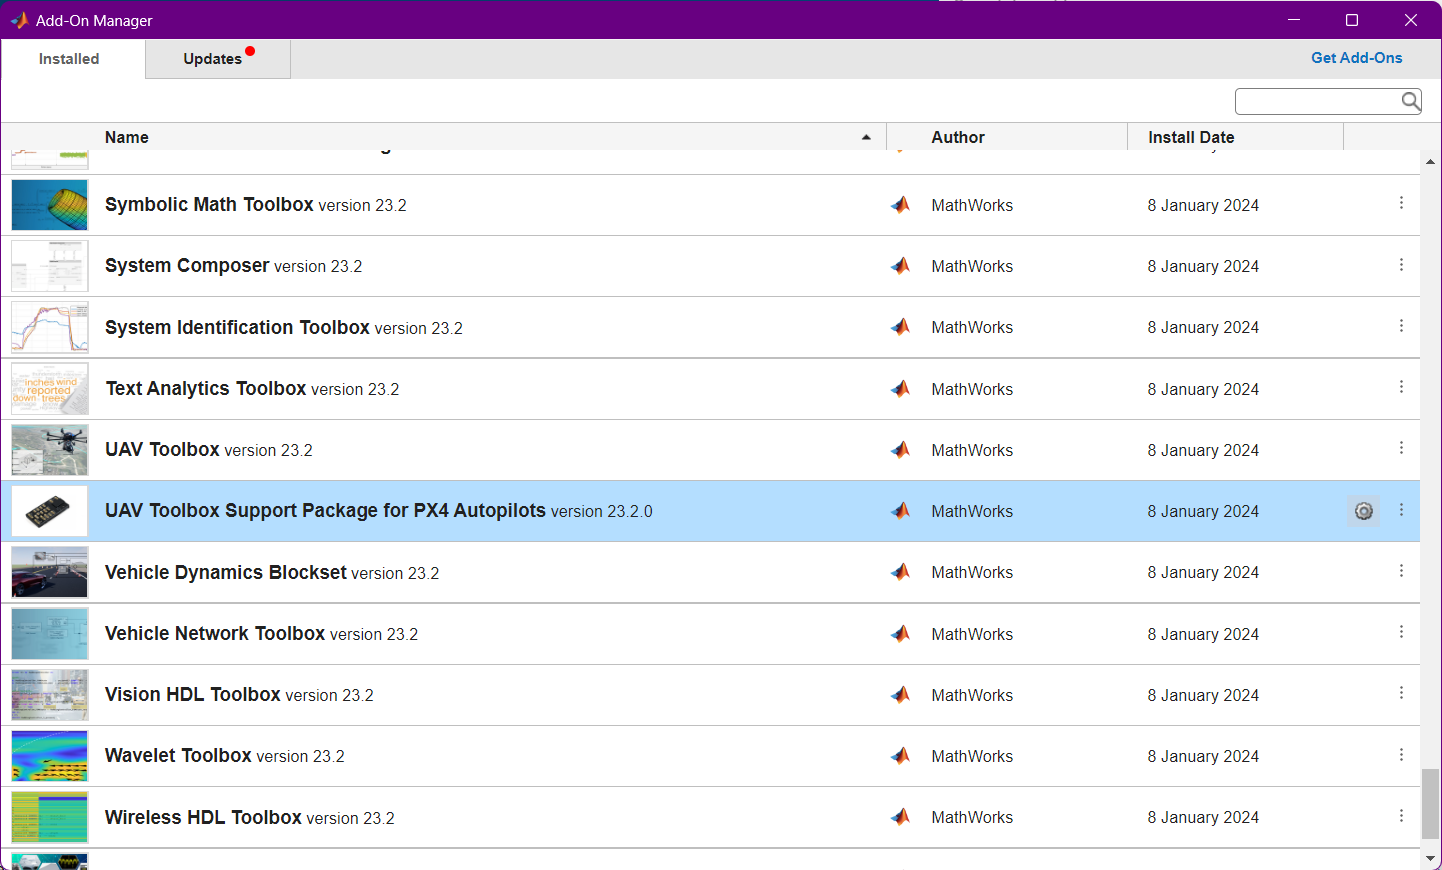
\includegraphics[width=\linewidth]{files/images/Screenshot 2024-03-13 120731.png} % Inserisci la seconda immagine
        \caption{Manage Toolbox}
        \label{fig:Manage Toolbox}
    \end{minipage}
\end{figure}

Una volta aperto l'Hardware Setup, inserire il percorso utilizzato per l'installazione del toolchain Cygwin (stesso percorso della Figura \ref{fig:Selezione della cartella di installazione}), quindi fare clic su Verifica Installazione (Fig. \ref{fig:Verifica Percorso}).
\begin{figure}[H] % Opzione [h] posiziona la figura qui (here)
  \centering
  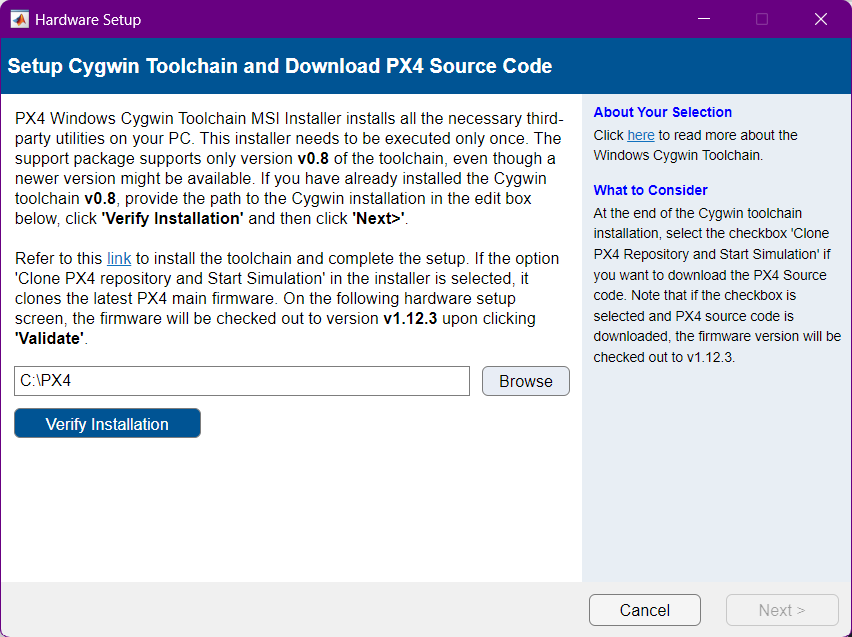
\includegraphics[width=0.7\textwidth]{files/images/matlab3.png} % Imposta la larghezza dell'immagine al 50% della larghezza del testo
  \caption{Verifica Percorso} % Didascalia sotto l'immagine
  \label{fig:Verifica Percorso} % Etichetta per fare riferimento all'immagine nel testo
\end{figure}
\noindent
Una volta uscita una spunta verde, clicca Next (Fig. \ref{fig:Verifica Percorso andata a buon fine}).
\begin{figure}[H] % Opzione [h] posiziona la figura qui (here)
  \centering
  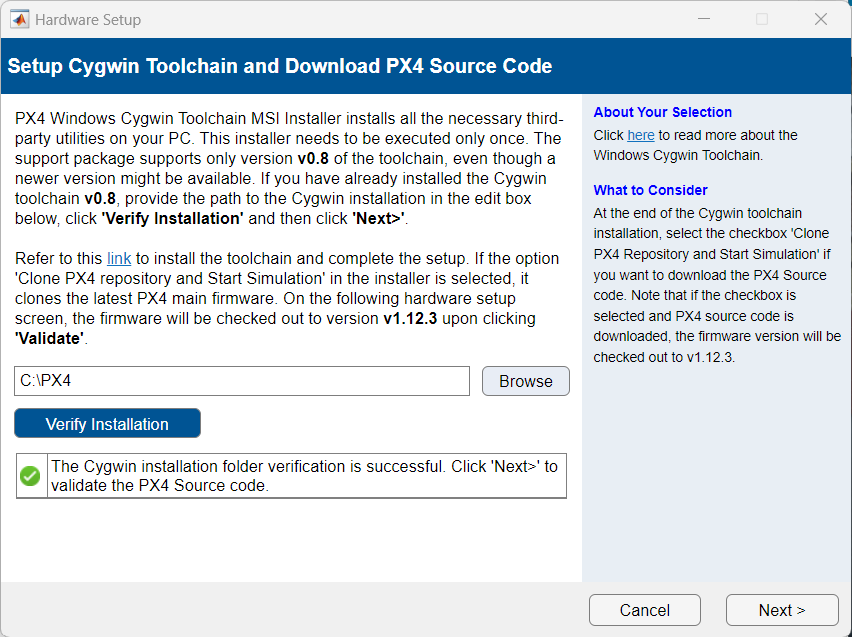
\includegraphics[width=0.7\textwidth]{files/images/matlab4.png} % Imposta la larghezza dell'immagine al 50% della larghezza del testo
  \caption{Verifica Percorso andata a buon fine} % Didascalia sotto l'immagine
  \label{fig:Verifica Percorso andata a buon fine} % Etichetta per fare riferimento all'immagine nel testo
\end{figure}
\noindent
Selezionare la cartella di download per il codice sorgente della PX4 (Fig. \ref{fig:Cartella di download per il codice sorgente della PX4}).
\begin{figure}[H] % Opzione [h] posiziona la figura qui (here)
  \centering
  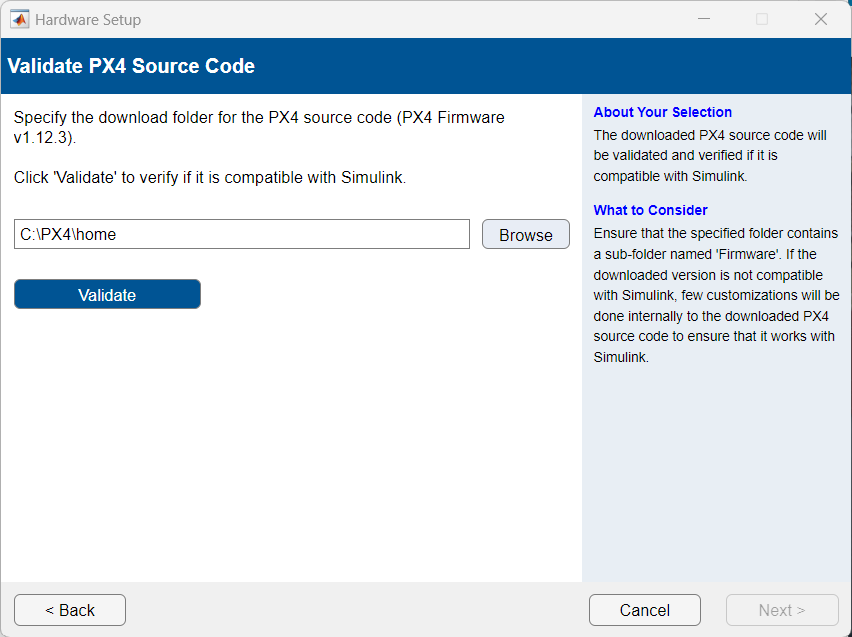
\includegraphics[width=0.7\textwidth]{files/images/matlab5.png} % Imposta la larghezza dell'immagine al 50% della larghezza del testo
  \caption{Cartella di download per il codice sorgente della PX4} % Didascalia sotto l'immagine
  \label{fig:Cartella di download per il codice sorgente della PX4} % Etichetta per fare riferimento all'immagine nel testo
\end{figure}
\noindent
Aspettare che esca la scritta "Firmware validation successful" e clicca "Next" (Fig. \ref{fig:Firmware validation successful}).
\begin{figure}[H] % Opzione [h] posiziona la figura qui (here)
  \centering
  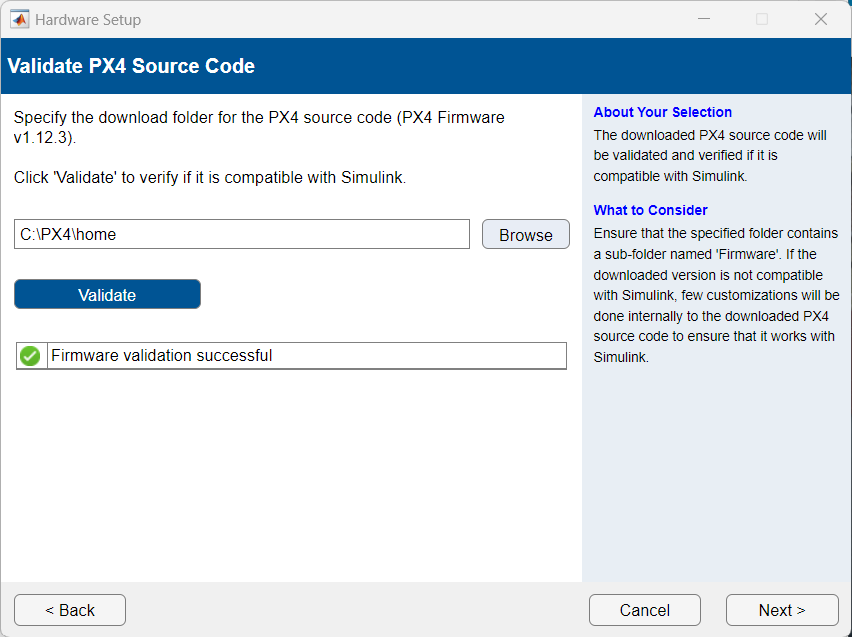
\includegraphics[width=0.7\textwidth]{files/images/matlab6.png} % Imposta la larghezza dell'immagine al 50% della larghezza del testo
  \caption{Firmware validation successful} % Didascalia sotto l'immagine
  \label{fig:Firmware validation successful} % Etichetta per fare riferimento all'immagine nel testo
\end{figure}
\noindent
Selezionare "Design Flight Controller in Simulink" e clicca "Next" (Fig. \ref{fig:Design Flight Controller in Simulink}) 
\begin{figure}[H] % Opzione [h] posiziona la figura qui (here)
  \centering
  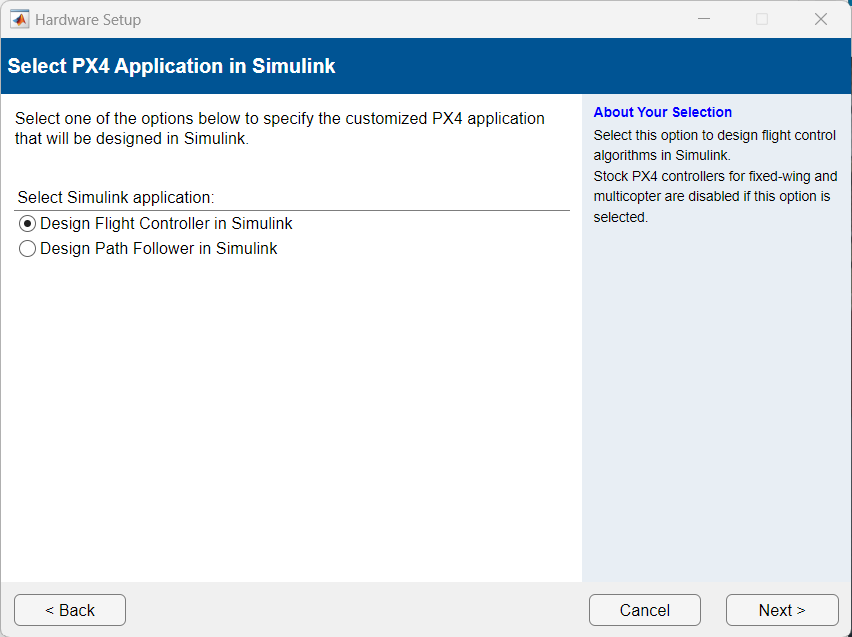
\includegraphics[width=0.7\textwidth]{files/images/matlab7.png} % Imposta la larghezza dell'immagine al 50% della larghezza del testo
  \caption{Design Flight Controller in Simulink} % Didascalia sotto l'immagine
  \label{fig:Design Flight Controller in Simulink} % Etichetta per fare riferimento all'immagine nel testo
\end{figure}
\noindent
Selezionare la "PX4 Pixhawk 6x" con build target "px4\_fmu\-v6x\_multicopter" e clicca "Next" (Fig. \ref{fig:Select a PX4 Autopilot and Build Target}).
\begin{figure}[H] % Opzione [h] posiziona la figura qui (here)
  \centering
  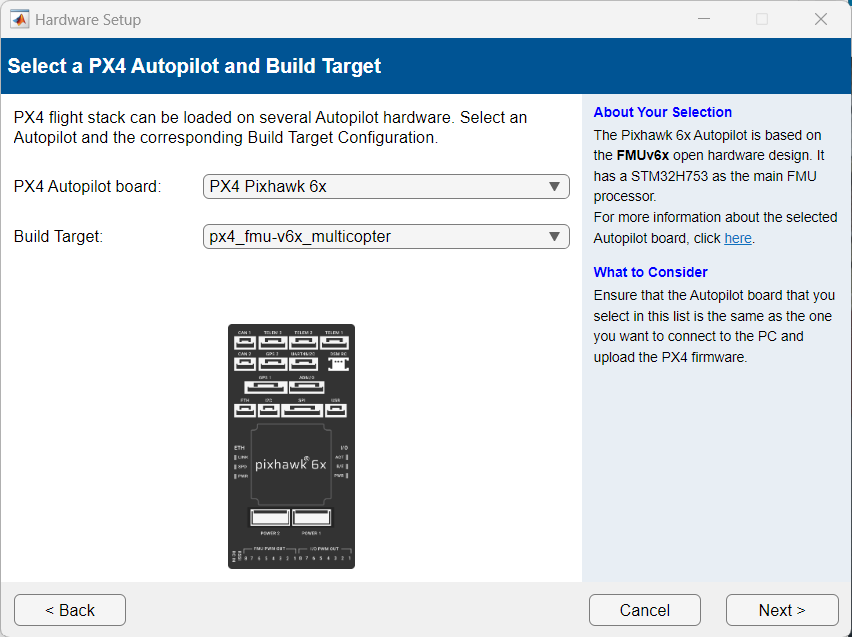
\includegraphics[width=0.7\textwidth]{files/images/matlab8.png} % Imposta la larghezza dell'immagine al 50% della larghezza del testo
  \caption{Select a PX4 Autopilot and Build Target} % Didascalia sotto l'immagine
  \label{fig:Select a PX4 Autopilot and Build Target} % Etichetta per fare riferimento all'immagine nel testo
\end{figure}
\noindent
Selezionare "Use default starup script" e clicca "Next" (Fig. \ref{fig:Select System Startup Script in PX4}).
\begin{figure}[H] % Opzione [h] posiziona la figura qui (here)
  \centering
  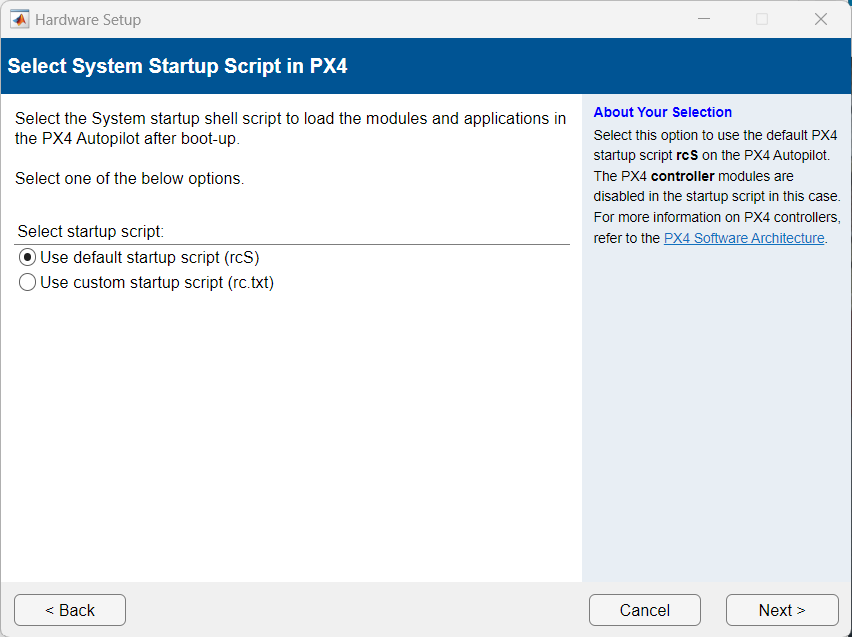
\includegraphics[width=0.7\textwidth]{files/images/matlab9.png} % Imposta la larghezza dell'immagine al 50% della larghezza del testo
  \caption{Select System Startup Script in PX4} % Didascalia sotto l'immagine
  \label{fig:Select System Startup Script in PX4} % Etichetta per fare riferimento all'immagine nel testo
\end{figure}
\noindent
Verificare la installazione di QGroundControl e cliccare "Next" (Fig. \ref{fig:Download QGroundControl} e Fig. \ref{fig:Download QGroundControl Successful}).
\begin{figure}[H] % Opzione [h] posiziona la figura qui (here)
  \centering
  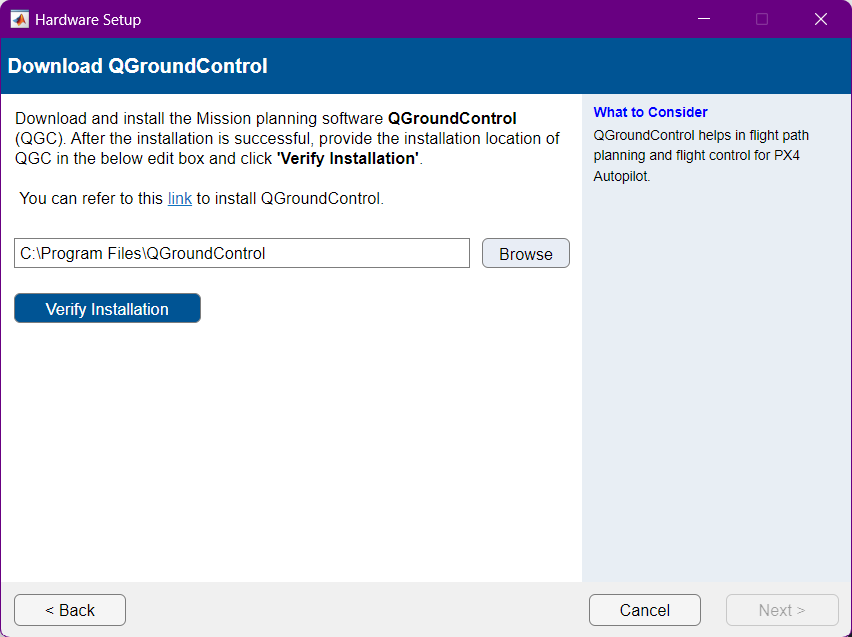
\includegraphics[width=0.7\textwidth]{files/images/matlab10.png} % Imposta la larghezza dell'immagine al 50% della larghezza del testo
  \caption{Download QGroundControl} % Didascalia sotto l'immagine
  \label{fig:Download QGroundControl} % Etichetta per fare riferimento all'immagine nel testo
\end{figure}
\noindent
\begin{figure}[H] % Opzione [h] posiziona la figura qui (here)
  \centering
  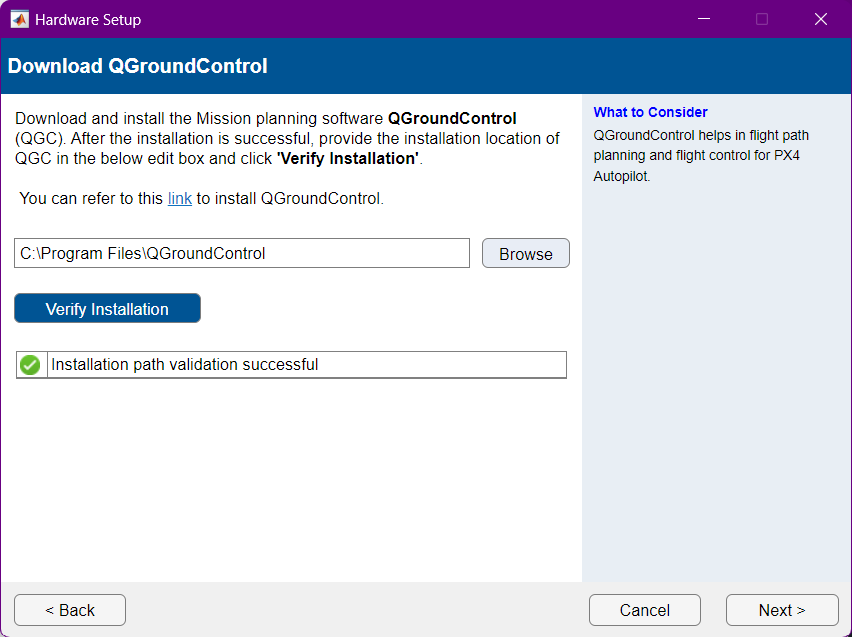
\includegraphics[width=0.7\textwidth]{files/images/matlab11.png} % Imposta la larghezza dell'immagine al 50% della larghezza del testo
  \caption{Download QGroundControl Successful} % Didascalia sotto l'immagine
  \label{fig:Download QGroundControl Successful} % Etichetta per fare riferimento all'immagine nel testo
\end{figure}
\noindent
Clicca "Next" (Fig. \ref{fig:Select Airframe in QGroundControl}).
\begin{figure}[H] % Opzione [h] posiziona la figura qui (here)
  \centering
  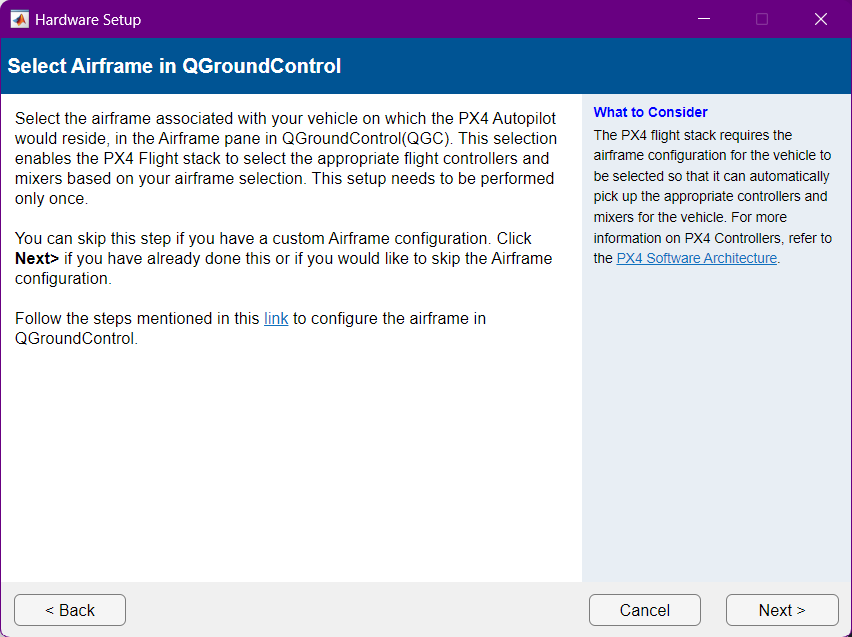
\includegraphics[width=0.7\textwidth]{files/images/matlab12.png} % Imposta la larghezza dell'immagine al 50% della larghezza del testo
  \caption{Select Airframe in QGroundControl} % Didascalia sotto l'immagine
  \label{fig:Select Airframe in QGroundControl} % Etichetta per fare riferimento all'immagine nel testo
\end{figure}
\noindent
Spuntere la casella "Delete PX4 Build folder for all CMake Configurations before building Firmware" ed eseguire il Build del Firmware (Fig. \ref{fig:Build Firmware}).
\begin{figure}[H] % Opzione [h] posiziona la figura qui (here)
  \centering
  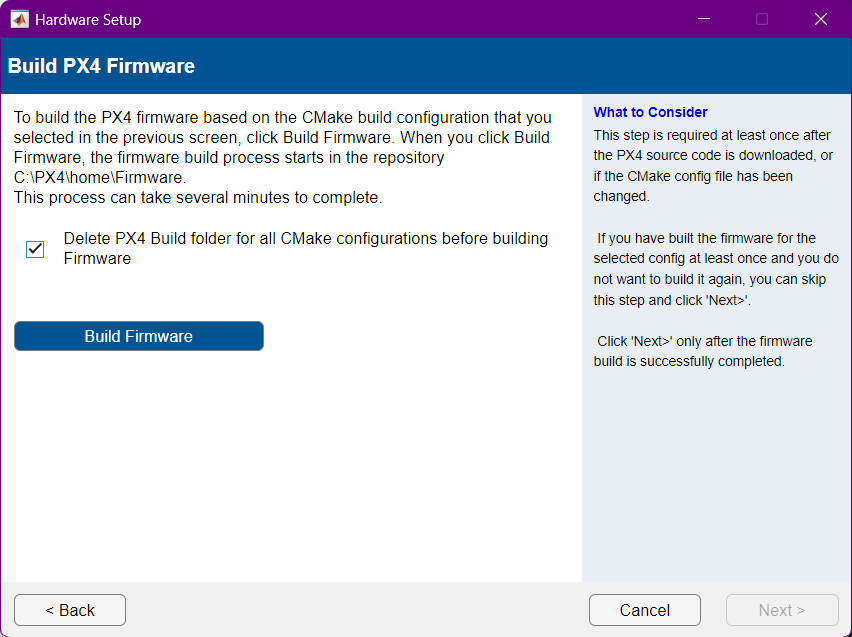
\includegraphics[width=0.7\textwidth]{files/images/matlab13.png} % Imposta la larghezza dell'immagine al 50% della larghezza del testo
  \caption{Build Firmware} % Didascalia sotto l'immagine
  \label{fig:Build Firmware} % Etichetta per fare riferimento all'immagine nel testo
\end{figure}
\noindent
Aspettare finchè non esce la scritta "Firmware Build Successful" e clicca "Next" (Fig. \ref{fig:Firmware Building} e Fig. \ref{fig:Firmware build successful}).
\begin{figure}[htbp]
    \begin{minipage}[b]{0.5\linewidth} % Definisci la larghezza della prima minipage (50% della larghezza della pagina)
      \centering
      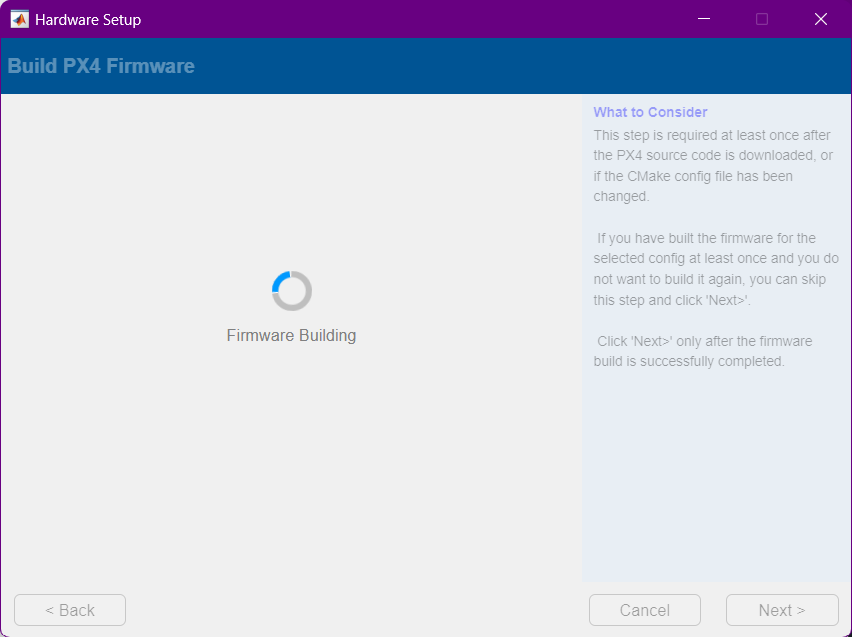
\includegraphics[width=\linewidth]{files/images/matlab14.png} % Imposta la larghezza dell'immagine al 50% della larghezza del testo
      \caption{Firmware Building} % Didascalia sotto l'immagine
      \label{fig:Firmware Building} % Etichetta per fare riferimento all'immagine nel testo
    \end{minipage}%
    \begin{minipage}[b]{0.5\linewidth} % Definisci la larghezza della seconda minipage (50% della larghezza della pagina)
        \centering
        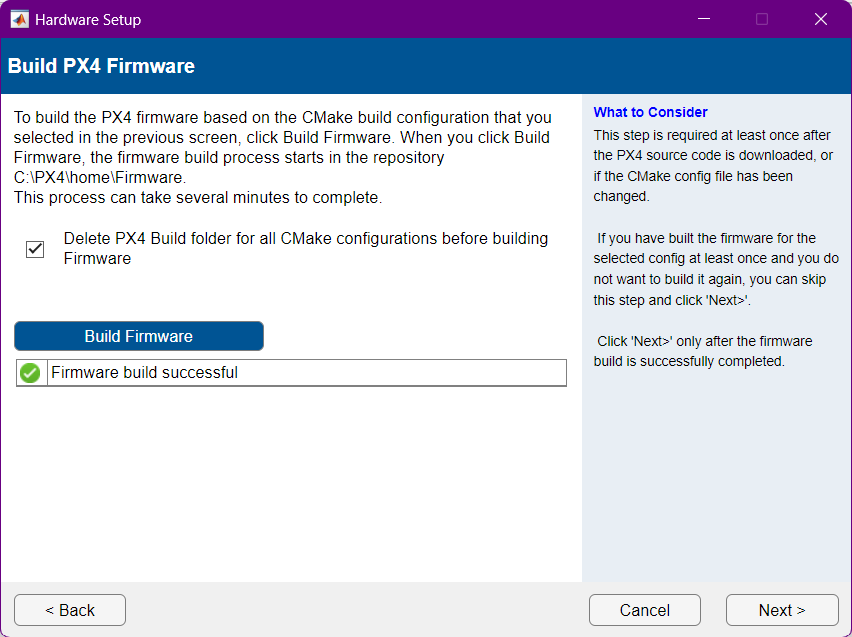
\includegraphics[width=\linewidth]{files/images/matlab15.png} % Imposta la larghezza dell'immagine al 50% della larghezza del testo
        \caption{Firmware build successful} % Didascalia sotto l'immagine
      \label{fig:Firmware build successful} % Etichetta per fare riferimento all'immagine nel
    \end{minipage}
\end{figure}
\noindent
Selezionare la COM a cui è collegata la PX4 ed eseguire il caricamento del firmware (Fig. \ref{fig:Test Connection}).
\begin{figure}[H] % Opzione [h] posiziona la figura qui (here)
  \centering
  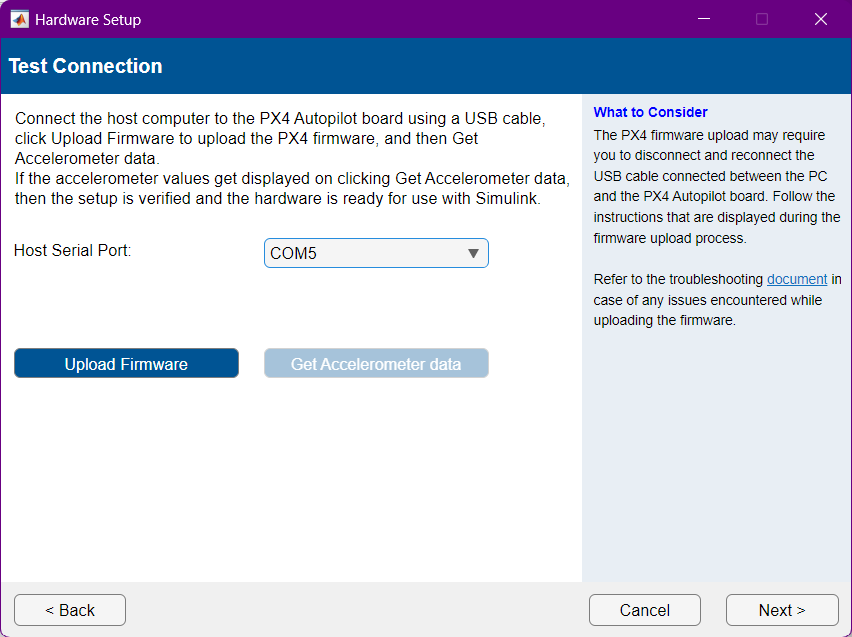
\includegraphics[width=0.7\textwidth]{files/images/matlab16.png} % Imposta la larghezza dell'immagine al 50% della larghezza del testo
  \caption{Test Connection} % Didascalia sotto l'immagine
  \label{fig:Test Connection} % Etichetta per fare riferimento all'immagine nel testo
\end{figure}
\noindent
Uscirà il messaggio mostrato in figura \ref{fig:Reconnect Pixhawk 6x}, clicca "OK" e scollegare la PX4 dal pc. Quindi togliere il cavo USB c e collegarlo nuovamente per il riavvio della PX4.
\begin{figure}[H] % Opzione [h] posiziona la figura qui (here)
  \centering
  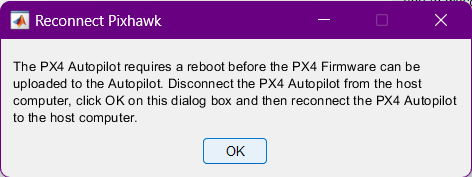
\includegraphics[width=0.7\textwidth]{files/images/matlab17.png} % Imposta la larghezza dell'immagine al 50% della larghezza del testo
  \caption{Reconnect Pixhawk 6x} % Didascalia sotto l'immagine
  \label{fig:Reconnect Pixhawk 6x} % Etichetta per fare riferimento all'immagine nel testo
\end{figure}
\noindent
A questo punto verrà effettuato il caricamento del firmware nella PX4, quindi aspettare il suo completamento (Fig. \ref{fig:Firmware uploading} e Fig. \ref{fig:Firmware upload successful}).


\begin{figure}[htbp]
    \begin{minipage}[b]{0.5\linewidth} % Definisci la larghezza della prima minipage (50% della larghezza della pagina)
      \centering
      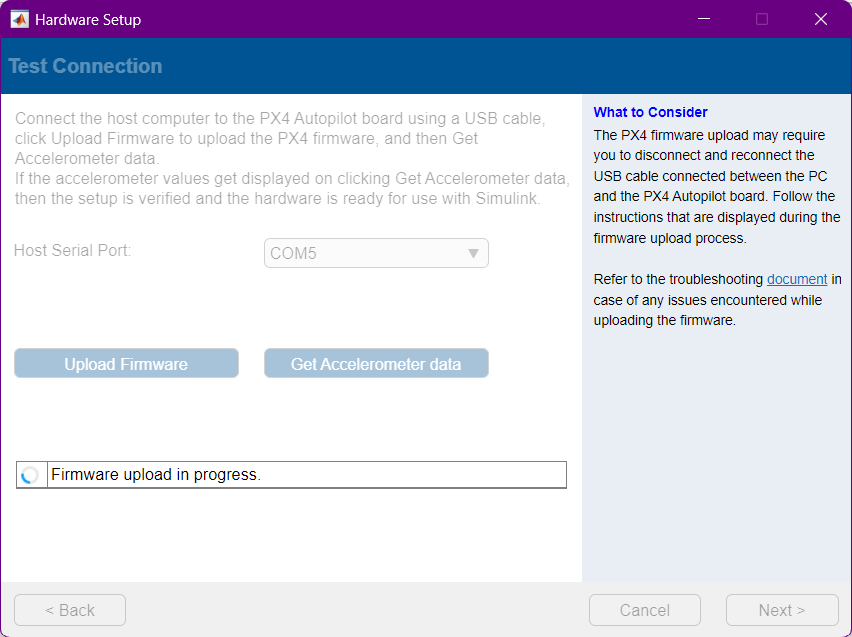
\includegraphics[width=\linewidth]{files/images/matlab18.png} % Imposta la larghezza dell'immagine al 50% della larghezza del testo
      \caption{Firmware uploading} % Didascalia sotto l'immagine
      \label{fig:Firmware uploading} % Etichetta per fare riferimento all'immagine nel testo
    \end{minipage}%
    \begin{minipage}[b]{0.5\linewidth} % Definisci la larghezza della seconda minipage (50% della larghezza della pagina)
        \centering
        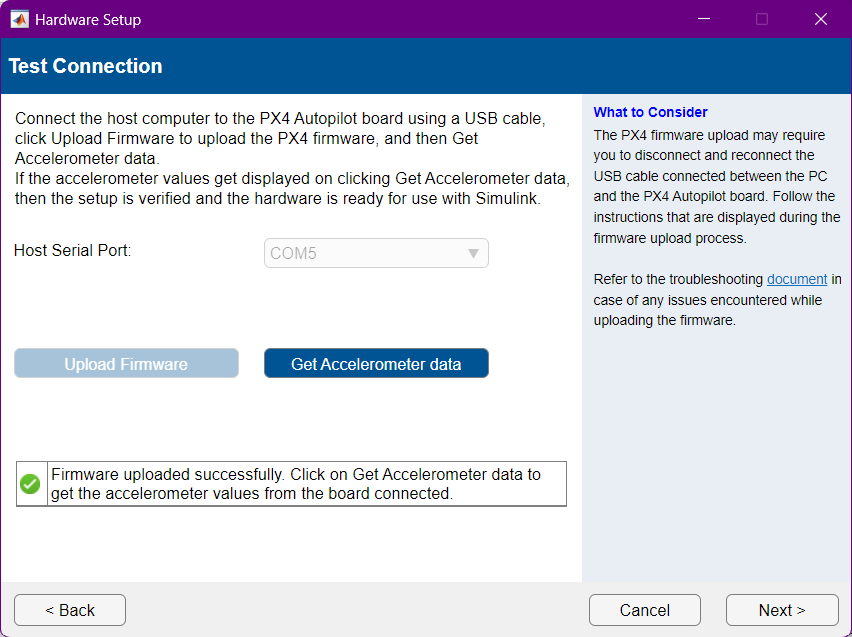
\includegraphics[width=\linewidth]{files/images/matlab19.png} % Imposta la larghezza dell'immagine al 50% della larghezza del testo
        \caption{Firmware upload successful} % Didascalia sotto l'immagine
      \label{fig:Firmware upload successful} % Etichetta per fare riferimento all'immagine nel
    \end{minipage}
\end{figure}
\noindent
A questo punto è terminata la configurazione del firmware per la PX4.

\section{Avvio Simulazione}
\subsection{Collegamento Hardware}
Come primo passo si collega la Pixhawk al computer host usando il cavo USB c, successivamente si collega la porta seriale a telem3 (/dev/ttyS7) e la porta USB sul computer host utilizzando un convertitore Serial-to-USB FTDI come mostrato nell'immagine di esempio qui sotto (Fig. \ref{fig:Collegamento PX4 Pixhawk 6x}).
\begin{figure}[H] % Opzione [h] posiziona la figura qui (here)
  \centering
  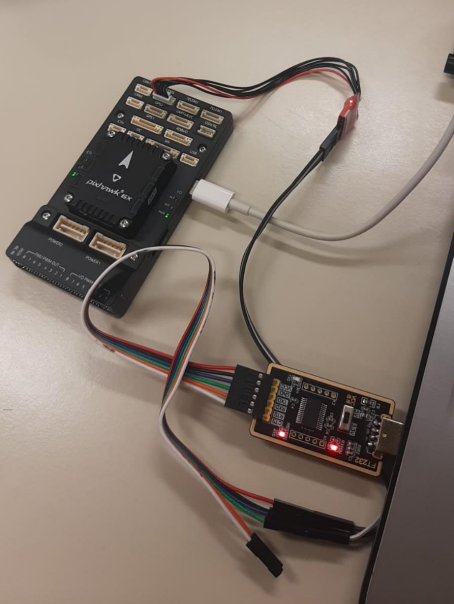
\includegraphics[width=0.5\textwidth]{files/images/collegamento_px4.png} % Imposta la larghezza dell'immagine al 50% della larghezza del testo
  \caption{Collegamento PX4 Pixhawk 6x} % Didascalia sotto l'immagine
  \label{fig:Collegamento PX4 Pixhawk 6x} % Etichetta per fare riferimento all'immagine nel testo
\end{figure}
\noindent


\subsection{Configurare il Modello}
 Una volta collegata la PX4, si va a configurare il modello Simulink e l'abilitazione per la calibrazione dei parametri negli strumenti di calibrazione di terze parti.
\\
Nota: Questi passaggi non sono necessari nel modello preconfigurato. Eseguire questi passaggi se hai modificato l'hardware o non stai utilizzando il modello preconfigurato.
\\
\begin{itemize}
    \item Apri il modello.
    \item Vai su Modeling > Model Settings per aprire la finestra di dialogo Configuration Parameters.
    \item Apri il pannello Hardware Implementation e seleziona la scheda PX4 Pixhawk 6x.
    \item Espandi le risorse hardware di destinazione per quella scheda.
    \item Fai clic su HITL e quindi seleziona Enable HITL Mode. Abilitando la modalità HITL, il simulatore jMAVSim e QGC vengono automaticamente configurati e avviati per essere eseguiti insieme al modello Simulink.
    \item Fai clic su External mode e seleziona /dev/ttyS7 come porta seriale della scheda hardware. Nel parametro Host Serial port, inserisci il numero di porta seriale host sul computer host per la comunicazione in modalità esterna.
    \item Fai clic su MAVLink e assicurati che sia selezionata l'opzione Enable MAVLink on /dev/ttyACM0.
    \item Fai clic su /dev/ttyS7 e imposta il Baud rate su 921600. Non modificare altri parametri.
    \item Fai clic su Apply e poi su OK.
\end{itemize}

\subsection{Avviare Monitor e Azione di Sintonizzazione per il Modello}
\begin{itemize}
    \item Nella scheda Hardware, nella sezione Mode, seleziona Run on board e poi fai clic su Monitor \& Tune.
    \item Questo avvia QGC
    \item In QGC, vai alla vista Plan.
    \item Crea una missione o carica la missione pre-pianificata, Mission.plan, disponibile con questo in figura \ref{fig:Test Volo with Unreal Enginee}.
    \begin{figure}[H] % Opzione [h] posiziona la figura qui (here)
      \centering
      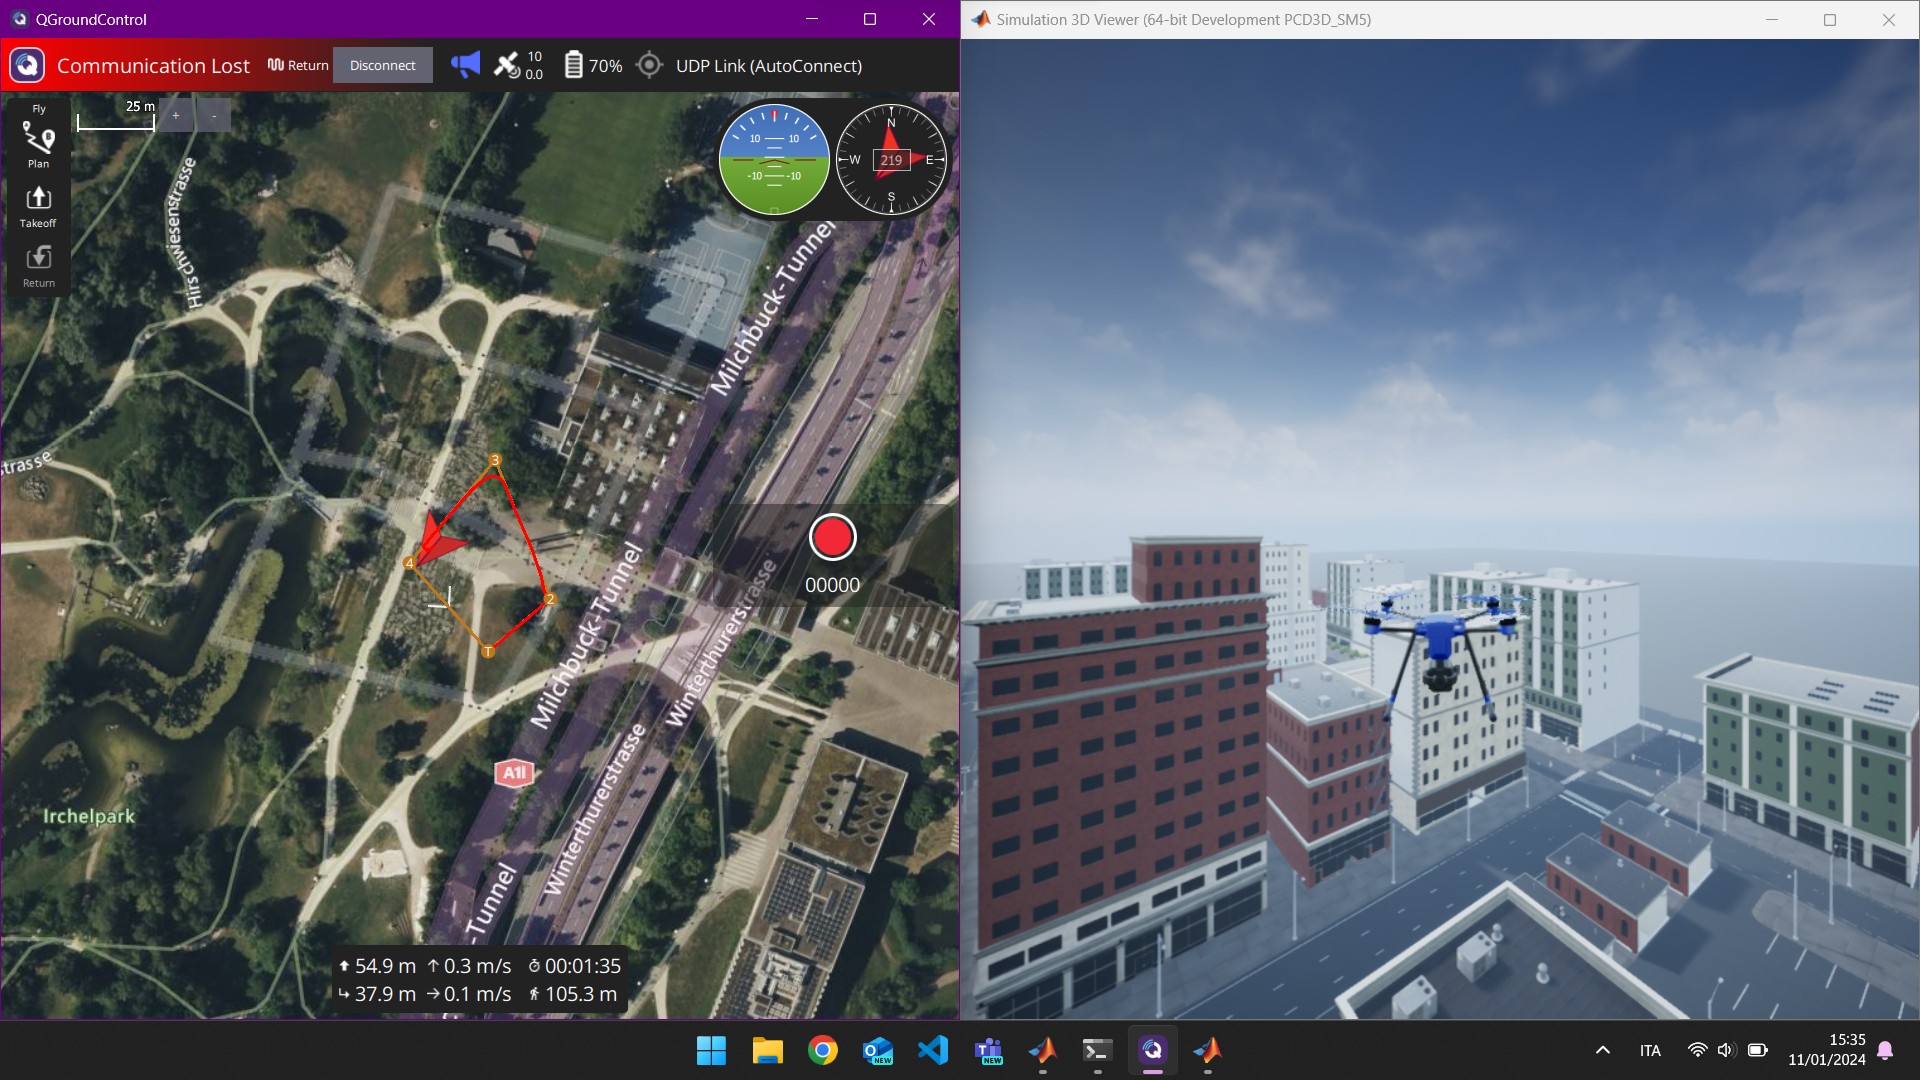
\includegraphics[width=0.8\textwidth]{files/images/test_volo.png} % Imposta la larghezza dell'immagine al 50% della larghezza del testo
      \caption{Test Volo with Unreal Enginee} % Didascalia sotto l'immagine
      \label{fig:Test Volo with Unreal Enginee} % Etichetta per fare riferimento all'immagine nel testo
    \end{figure}
\noindent
    \item Crea una missione: Per informazioni su come creare una missione, consulta Plan View.
    \item Carica una missione: Fai clic su Open Example nella parte superiore di questa pagina per salvare il file di piano sul tuo computer. Dopo aver salvato il file .plan, avvia QGC, e fai clic su File > Open per caricare il piano su QGC. Dopo aver caricato il piano, la missione è visibile in QGC.
    \item Fai clic sul pulsante Upload nell'interfaccia QGC per caricare la missione da QGroundControl.
    \\
    Nota: Se la scheda hardware viene riavviata dopo che la missione è stata caricata, la missione potrebbe non funzionare se QGC, UAV Dynamics e 3D Visualization with Unreal Engine del modello Simulink sono aperti. Riavvia QGC, UAV Dynamics e 3D Visualization with Unreal Engine, successivamente carica nuovamente la missione per risolvere il problema.
    \\
    \item Vai alla vista Fly per visualizzare la missione caricata.
    \item Avvia la Missione in QGC. Dopo l'avvio della missione, il drone decolla e segue l'insieme di waypoints da QGC.
\end{itemize}

\subsection{Prova volo simulazione}
Di seguito sono elencati i segnali che sono stati registrati durante la simulazione:
\begin{itemize}
    \item PWM Motori
    \item Posizione (X, Y, Z)
    \item Angoli di Eulero (Yaw, Pitch, Roll)
    \item Velocità Lineare (dx, dy, dz)
    \item Accelerazione Lineare (ddx, ddy, ddz)
    \item Velocità Angolare (p, q, r)
\end{itemize}

Per il salvataggio dei segnali, al fine di analizzare in dettaglio le dinamiche del drone, sono stati integrati due blocchi To Workspace nel modello UAV Dynamics in Simulink. Questi blocchi sono stati inseriti per salvare le serie temporali nel workspace di MATLAB, in modo da poter elaborare i dati successivamente. Il modello Simulink in questione verrà visto in dettaglio nel capitolo successivo.


\subsection{Procedure Post-Simulazione e Visualizzazione dei Dati}

Dopo aver impostato il percorso della simulazione e avviato il processo, il successivo passo consiste nell'attendere il termine della simulazione per esaminare i dati acquisiti e valutare le prestazioni del drone. Questa fase comporta l'utilizzo di uno script in MATLAB, il quale facilita l'analisi, la visualizzazione e la conservazione dei dati ottenuti. Di seguito è formalizzata questa procedura:

\begin{enumerate}
    \item \textbf{Termine della Simulazione:}
    \begin{itemize}
        \item Una volta avviata la simulazione, si attende il termine del processo per garantire che tutti i dati rilevanti siano stati registrati nel workspace (Fig. \ref{fig:Percorso di prova}).
        \begin{figure}[htbp]
            \begin{minipage}[b]{0.5\linewidth} % Definisci la larghezza della prima minipage (50% della larghezza della pagina)
              \centering
              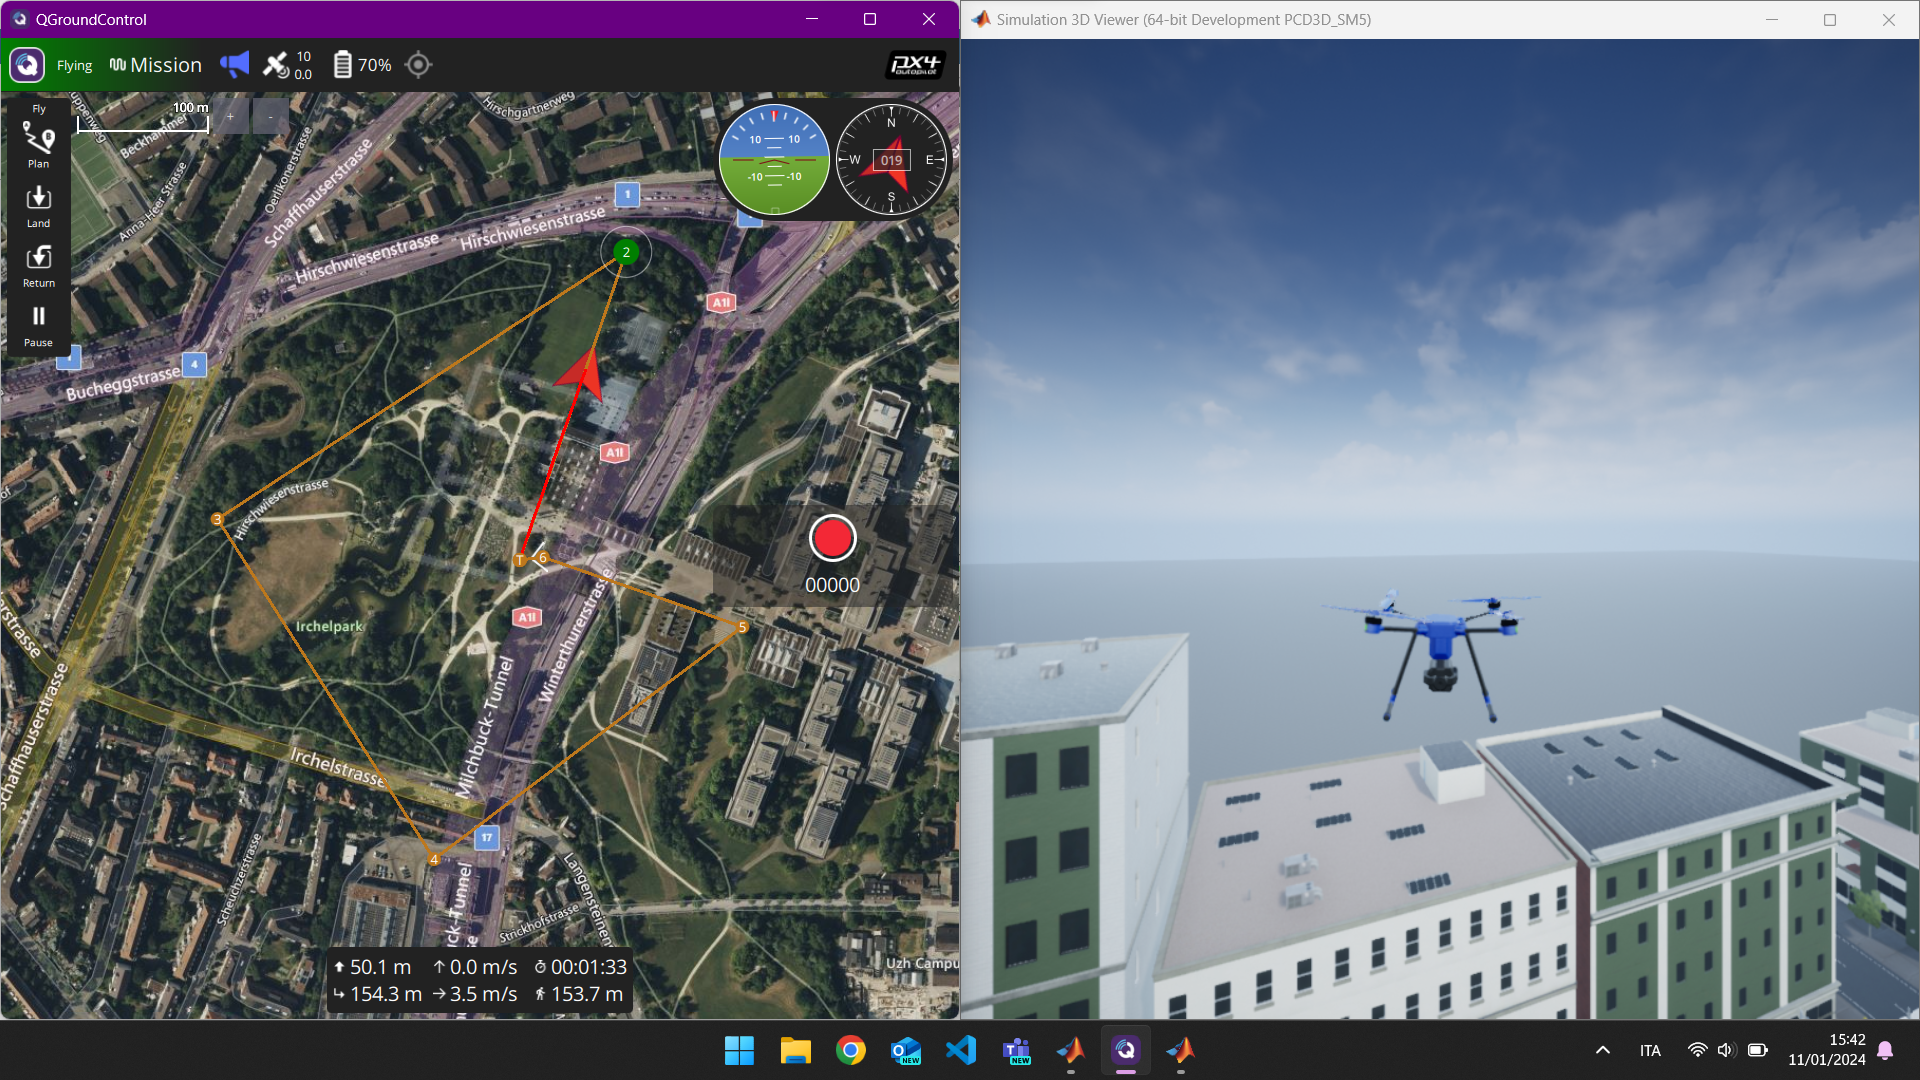
\includegraphics[width=\linewidth]{files/images/path1.png} % Imposta la larghezza dell'immagine al 50% della larghezza del testo
            \end{minipage}%
            \begin{minipage}[b]{0.5\linewidth} % Definisci la larghezza della seconda minipage (50% della larghezza della pagina)
                \centering
                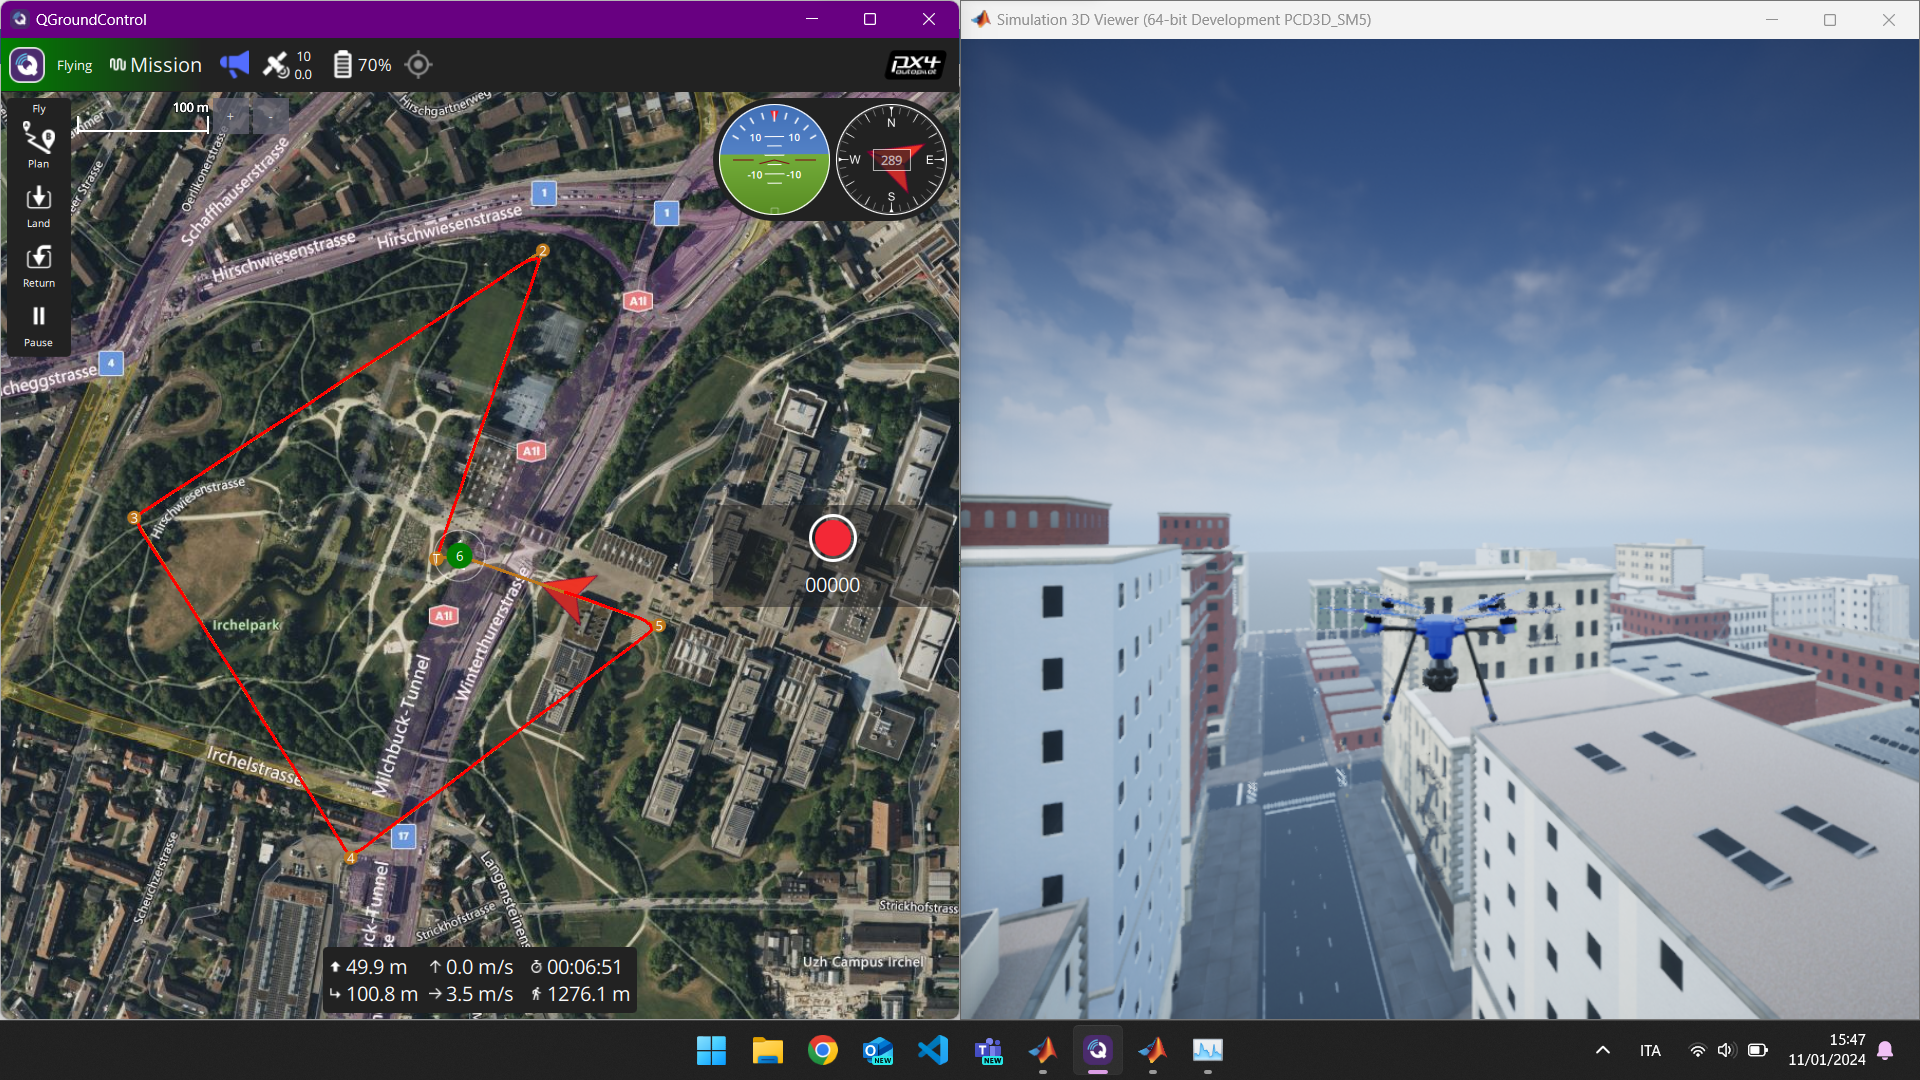
\includegraphics[width=\linewidth]{files/images/path1_finish.png} % Imposta la larghezza dell'immagine al 50% della larghezza del testo
            \end{minipage}
            \caption{Percorso di prova}
            \label{fig:Percorso di prova}
        \end{figure}
        
    \end{itemize}

    \item \textbf{Salvataggio e plot dati:}
    \begin{itemize}
        \item Dopo la conclusione della simulazione, uno script MATLAB preconfigurato viene eseguito per automatizzare il processo di visualizzazione e salvataggio dei dati in un file .mat.
        \item Questi dati includono informazioni vitali quali PWM motori, posizione (X, Y, Z), angoli di Eulero, velocità lineare, accelerazione lineare e velocità angolare.
        \item Lo script genera esegue il plot di ciascuna serie temporale. Questi grafici offrono una visione chiara e dettagliata delle dinamiche del drone durante la simulazione.
    \end{itemize}

    \item \textbf{Plot 3D del Percorso:}
    \begin{itemize}
        \item Utilizzando le informazioni sulla posizione (X, Y, Z) precedentemente registrate, un ulteriore script in MATLAB genera un plot tridimensionale del percorso seguito dal drone durante la simulazione. Questo plot consente di confrontare visivamente il percorso effettivamente percorso con quello inizialmente impostato (Fig. \ref{fig:Plot3D}).
        \begin{figure}[htbp]
            \begin{minipage}[b]{0.5\linewidth} % Definisci la larghezza della prima minipage (50% della larghezza della pagina)
              \centering
              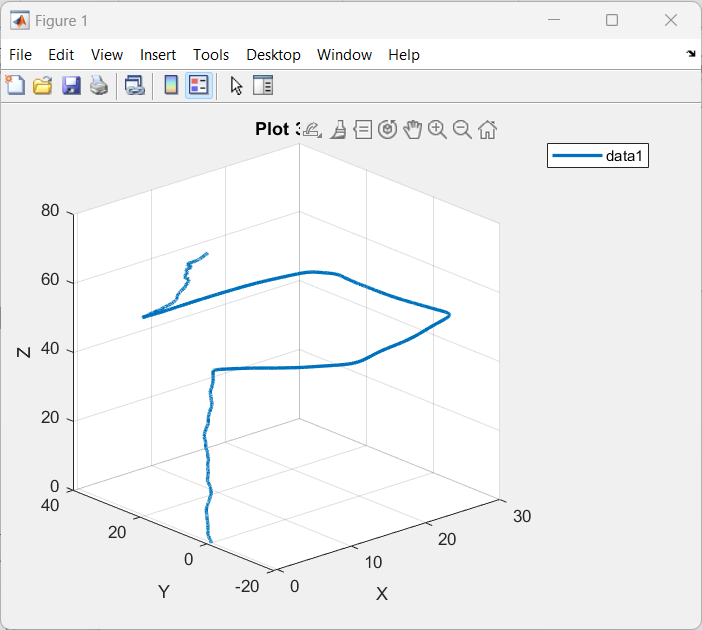
\includegraphics[width=\linewidth]{files/images/plot3D.png} % Imposta la larghezza dell'immagine al 50% della larghezza del testo
            \end{minipage}%
            \begin{minipage}[b]{0.5\linewidth} % Definisci la larghezza della seconda minipage (50% della larghezza della pagina)
                \centering
                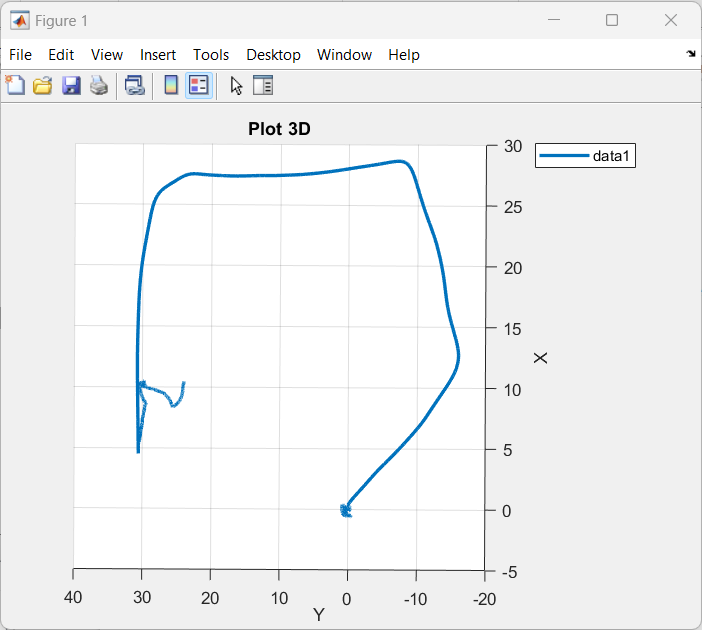
\includegraphics[width=\linewidth]{files/images/plot3D_1.png} % Imposta la larghezza dell'immagine al 50% della larghezza del testo
            \end{minipage}
            \caption{Plot 3D}
            \label{fig:Plot3D}
        \end{figure}
    \end{itemize}

    
\end{enumerate}








 \clearemptydoublepage
\chapter{Modello Matlab/Simulink} \clearemptydoublepage
\chapter{Inserimento guasti e Rilevamento}

Nella prima fase del nostro studio, abbiamo implementato una strategia di rilevamento del guasto al motore mediante la modifica dei valori PWM utilizzando Simulink. Questo è stato eseguito nel blocco "Quadcopter Model" nel file Simulink "UAV Dynamics" (Figura \ref{fig:guasto PWM}).
\begin{figure}[H]  % 'H' forza la posizione esatta
    \centering
    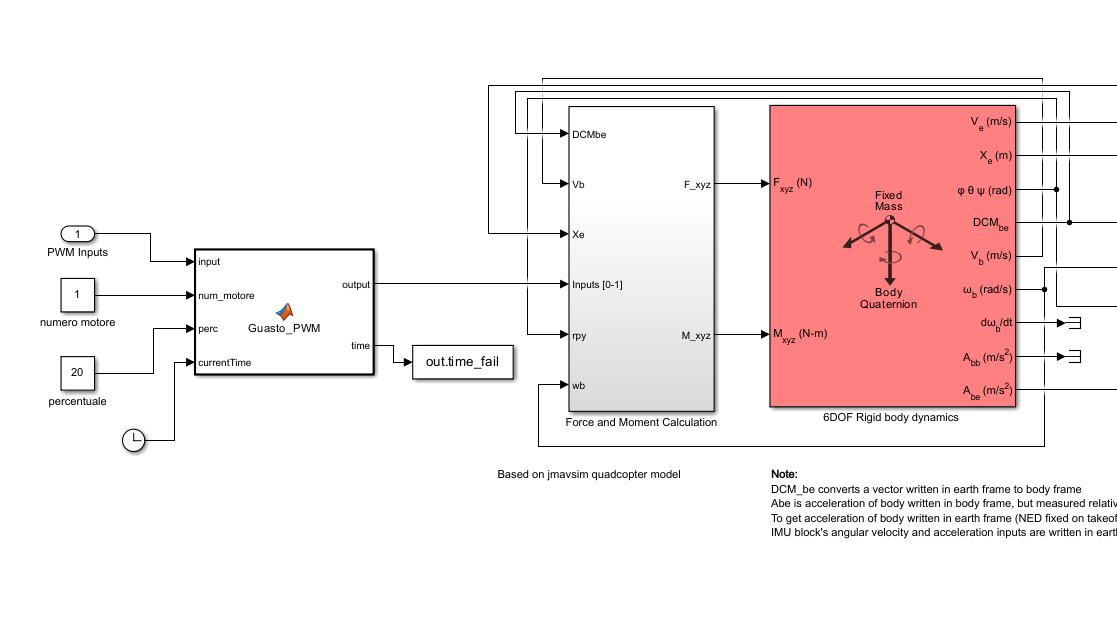
\includegraphics[width=0.8\textwidth]{guasto_pwm.png}
    \caption{Blocco Guasto PWM}
    \label{fig:guasto PWM}
\end{figure}
\noindent
Abbiamo introdotto una funzione MATLAB all'interno del blocco "matlab\_function", la quale prende in input il numero del motore interessato, la percentuale di guasto da applicare al PWM e il tempo corrente.

\begin{lstlisting}[language=Matlab, caption={Funzione MATLAB per il rilevamento del guasto PWM}, label=lst:guasto_pwm]
function [output, time] = Guasto_PWM(input, num_motore, 
perc, currentTime)   
    if num_motore == 0
        output = input;
        time = 0;
    else
        % Copia i valori di PWM in una variabile temporanea
        output = input;
        % Diminuisci il % del valore del PWM del motore 
        specificato
        output(num_motore) = (100 - perc) / 100 * 
        output(num_motore);
        % Ottieni istante inserimento guasto
        time = currentTime;
    end
end
\end{lstlisting}
\noindent

Nella funzione mostrata nel listato~\ref{lst:guasto_pwm}, consente di simulare il guasto riducendo la percentuale di PWM del motore specificato. 

\begin{figure}[H]  % 'H' forza la posizione esatta
    \centering
    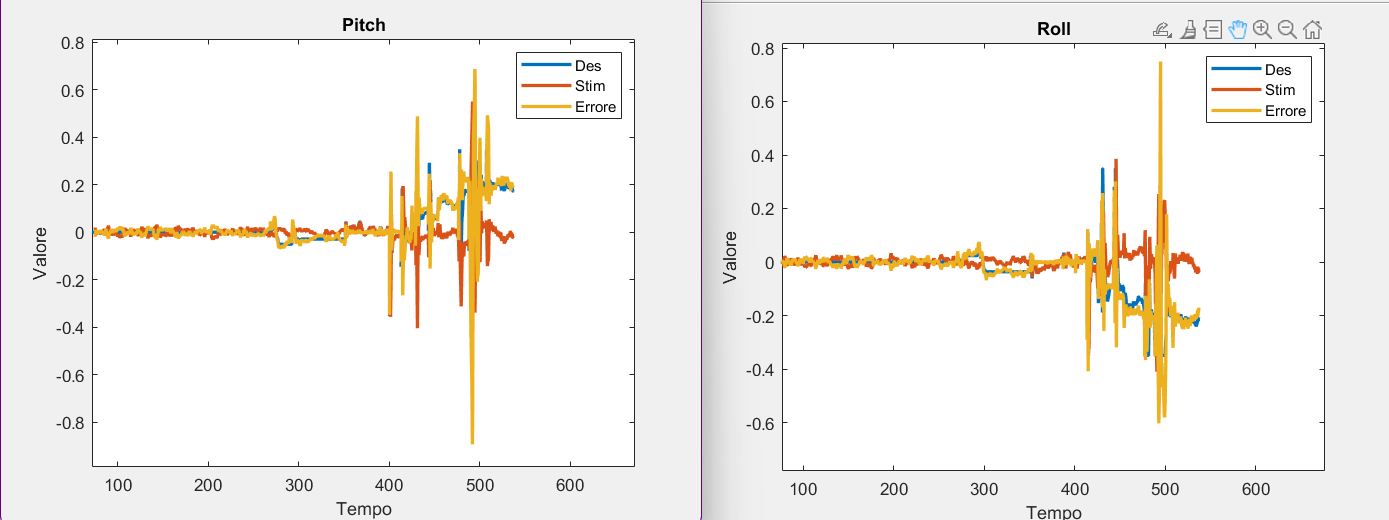
\includegraphics[width=0.9\textwidth]{pitch_roll.png}
    \caption{Andamento Angoli di Eulero Pitch e Roll con guasto al 20\% sul PWM del motore 1}
    \label{fig:pitch_roll}
\end{figure}

\noindent
Dopo aver introdotto un guasto in uno dei motori durante il volo del drone e aver eseguito una curva, abbiamo notato che l'errore tra gli angoli desiderati e stimati di pitch e roll assumeva valori diversi da zero (Figura \ref{fig:pitch_roll}). 
\noindent
Questa osservazione ha costituito la base per lo sviluppo degli algoritmi di rilevamento del guasto successivi.

\section{Rilevamento dei Guasti tramite Soglia Fissa}

Nella fase successiva del nostro studio, ci siamo concentrati sullo sviluppo di un algoritmo di rilevamento dei guasti tramite soglia fissa. Questo approccio si basa sull'osservazione della variazione dell'errore degli angoli di pitch e roll dopo l'inserimento di un guasto su uno dei motori del drone. L'errore era calcolato confrontando l'angolo desiderato con quello stimato (eq. \ref{eq:pitch_error} ed eq. \ref{eq:roll_error}) . Abbiamo notato che questa variazione dipendeva dal motore interessato dal guasto.
\begin{equation}
\text{Errore di pitch} = \text{Angolo desiderato di pitch} - \text{Angolo stimato di pitch}
\label{eq:pitch_error}
\end{equation}
\begin{equation}
\text{Errore di roll} = \text{Angolo desiderato di roll} - \text{Angolo stimato di roll}
\label{eq:roll_error}
\end{equation}
\noindent
La rilevazione dei guasti avviente dentro al FlightController, quindi all'interno del file Simulink "Quadcopter\_ControllerWithNavigation" sono stati inseriti i seguenti blocchi mostrati in figura \ref{fig:Blocchi per il rilevamento a soglia fissa con buffer}.

\begin{figure}[H]  % 'H' forza la posizione esatta
    \centering
    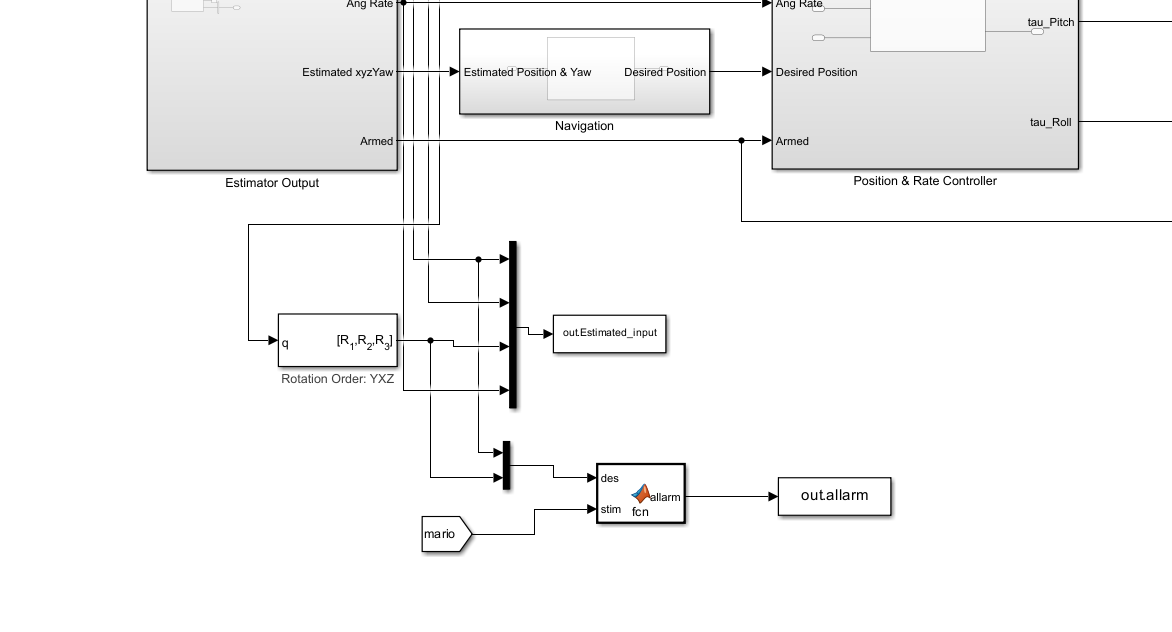
\includegraphics[width=0.9\textwidth]{files/images/soglia_fissa_buffer.png}
    \caption{Blocchi per il rilevamento a soglia fissa con buffer in Quadcopter\_ControllerWithNavigation}
    \label{fig:Blocchi per il rilevamento a soglia fissa con buffer}
\end{figure}
\noindent
Per implementare l'algoritmo di rilevamento dei guasti, abbiamo definito delle soglie fisse sugli errori degli angoli di pitch e roll. Durante la fase di volo del drone, abbiamo monitorato costantemente gli errori degli angoli di pitch e roll e abbiamo confrontato i loro valori con le soglie fissate. Quando entrambi gli errori di  dei valori superava la soglia prestabilita, scattava un allarme indicando il motore affetto dal guasto.
\\
Per aumentare l'efficienza del rilevamento, abbiamo utilizzato un buffer di campionamento. Ogni volta che veniva rilevata una variazione sugli angoli di pitch e roll, registravamo i valori degli angoli per un numero prefissato di campioni, ad esempio 500 (equivale ad un campionamento di 5 secondi). Successivamente, calcolavamo la media degli angoli registrati e confrontavamo questa media con le soglie fisse. Se la media superava una delle soglie, l'allarme di guasto veniva attivato. Il seguente è il codice all'interno del blocco funzione MATLAB, mostrato in figura \ref{fig:Blocchi per il rilevamento a soglia fissa con buffer}, per la rilevazione guasti.
\begin{lstlisting}[language=Matlab, caption={Descrizione del codice}, label={lst:codice_matlab}]
function allarm = fcn(stim, des)
    persistent PitchBuffer RollBuffer
    if isempty(PitchBuffer)
        PitchBuffer = zeros(1, 500);
        RollBuffer = zeros(1, 500);
    end

    % Calcolo gli errori di Pitch e Roll
    Pitch_Error = des(2) - stim(2);
    Roll_Error = des(3) - stim(3);

    % Per evitare che la media dia errore per i NaN, 
    sostituisco con 0
    if(isnan(Pitch_Error) && isnan(Roll_Error))
       Pitch_Error = 0;
       Roll_Error = 0;
    end

    % Aggiorna i buffer
    PitchBuffer = [PitchBuffer(2:end), Pitch_Error];
    RollBuffer = [RollBuffer(2:end), Roll_Error];

    % Soglie fisse
    PitchThreshold = 0.1;
    RollThreshold = 0.1;

    % Guasto Motore 1 del -20%
    if (mean(PitchBuffer) > PitchThreshold && 
    mean(RollBuffer) < -RollThreshold)
        allarm = 1;
    % Guasto Motore 2 del -20%
    elseif (mean(PitchBuffer) < -PitchThreshold && 
    mean(RollBuffer) > RollThreshold)
        allarm = 2;
    % Guasto Motore 3 del -20%
    elseif (mean(PitchBuffer) > PitchThreshold && 
    mean(RollBuffer) > RollThreshold)
        allarm = 3;
    % Guasto Motore 4 del -20%
    elseif (mean(PitchBuffer) < -PitchThreshold && 
    mean(RollBuffer) < -RollThreshold)
        allarm = 4;
    else
        allarm = 0;
    end
end
\end{lstlisting}
\noindent
Abbiamo osservato che l'approccio di rilevamento dei guasti tramite soglia fissa si è dimostrato efficace nel rilevare guasti durante la prima curva effettuata dal drone.
\\
Il percorso utilizzato per il test di volo con rilevamento guasto a soglia fissa è mostrato in Figura \ref{fig:Percorso Test Soglia Fissa con Buffer}. Durante ogni volo, il guasto è stato inserito tra il punto 7 e il punto 8 del percorso. Si sono ottenuti risultati distinti inserendo il guasto su ciascun motore durante i test.

\begin{figure}[H]
    \centering
    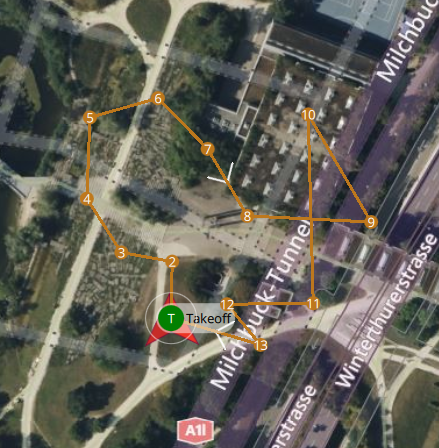
\includegraphics[width=0.5\textwidth]{files/images/path_soglia_fissa1 (1).png}
    \caption{Percorso Test Soglia Fissa con Buffer}
    \label{fig:Percorso Test Soglia Fissa con Buffer}
\end{figure}
\noindent
Ogni test ha prodotto risultati soddisfacenti, poiché non sono stati riscontrati falsi positivi e i falsi negativi sono stati osservati solamente nel tratto compreso tra l'inserimento del guasto e la prima curva da effettuare.

\begin{figure}[H]
    \centering
    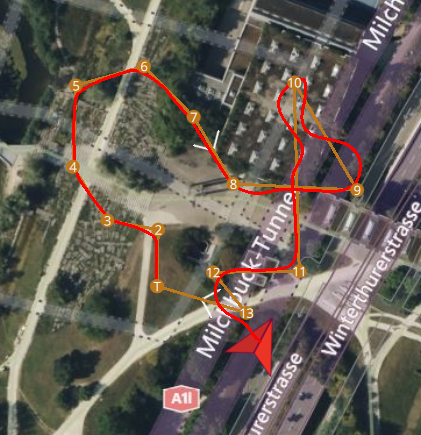
\includegraphics[width=0.5\textwidth]{files/images/path_soglia_fissa1 (2).png}
    \caption{Andamento del drone del test volo con guasto su potenza motore del 20\% su motore 1}
    \label{Risultato volo con guasto su potenza motore del 20\% su motore 1}
\end{figure}
\noindent

\begin{figure}[H]
    \centering
    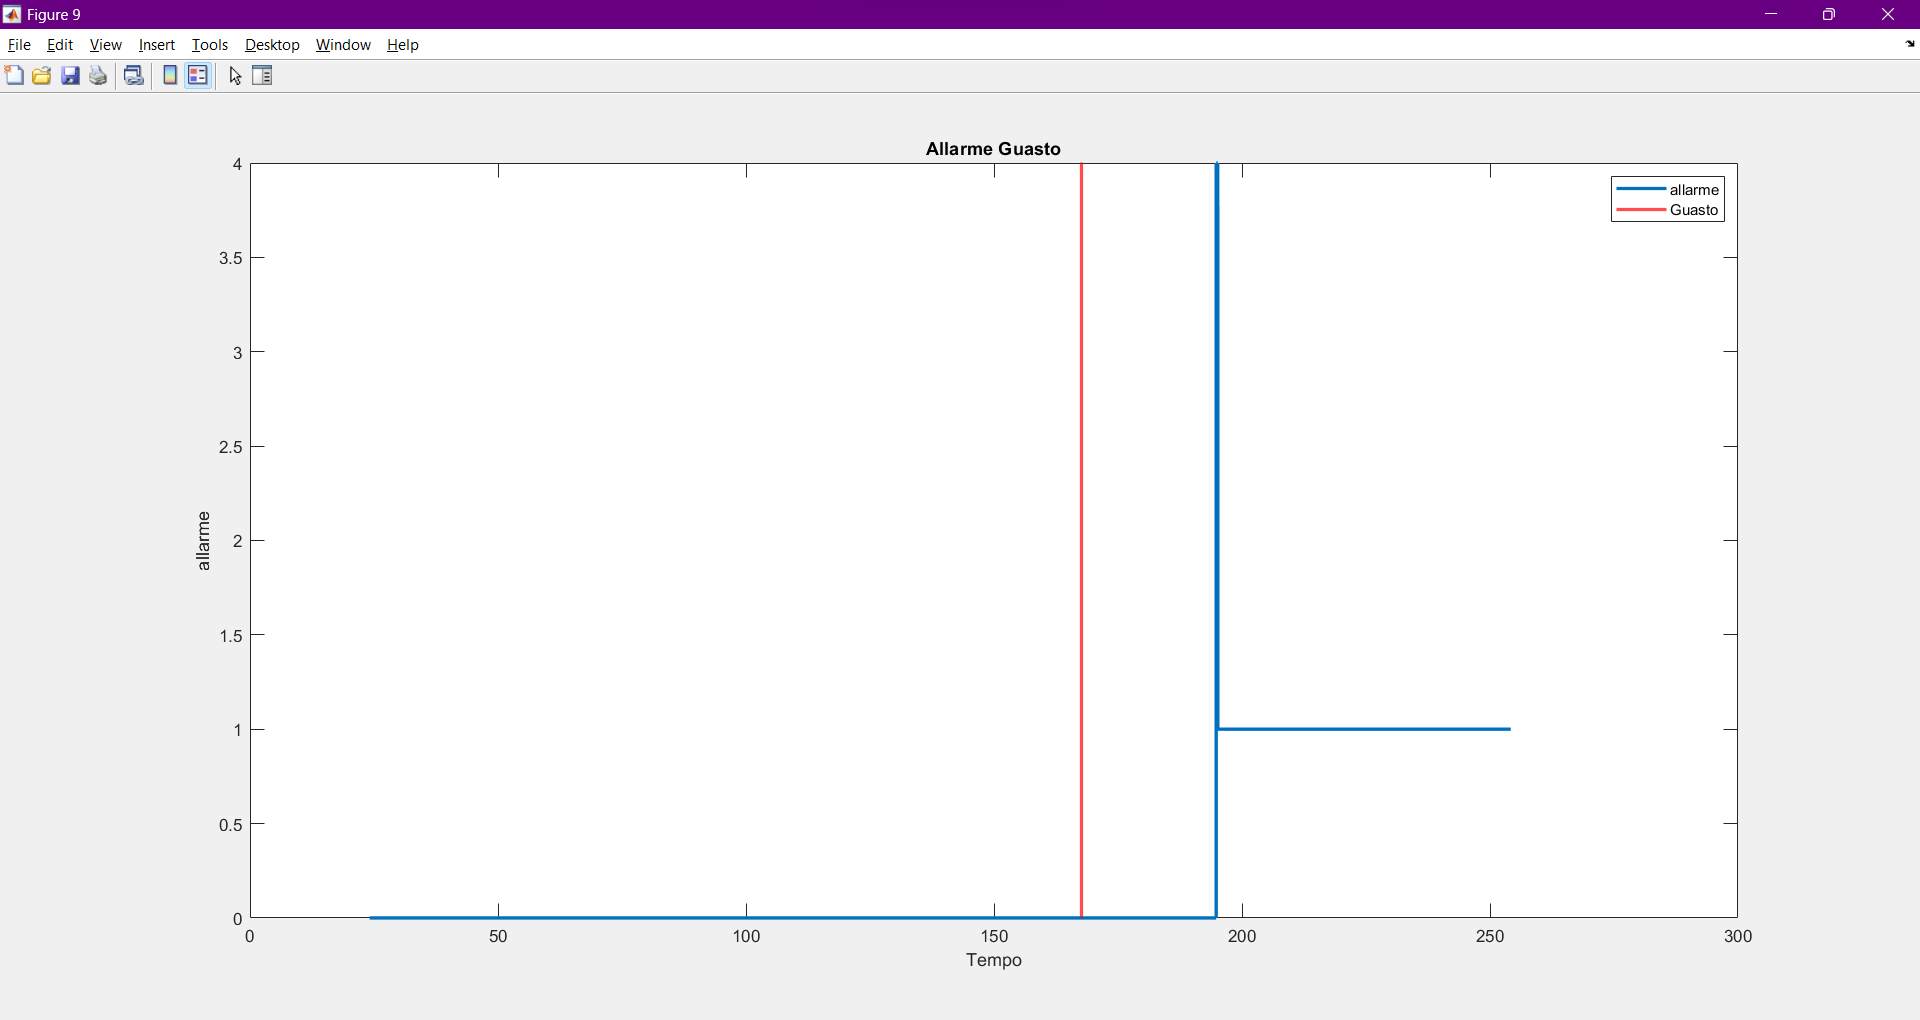
\includegraphics[width=\textwidth]{files/images/path_soglia_fissa1 (3).png}
    \caption{Allarmi del test volo con guasto su potenza motore del 20\% su motore 1}
    \label{Allarmi del test volo con guasto su potenza motore del 20\% su motore 1}
\end{figure}
\noindent

\begin{figure}[H]
    \centering
    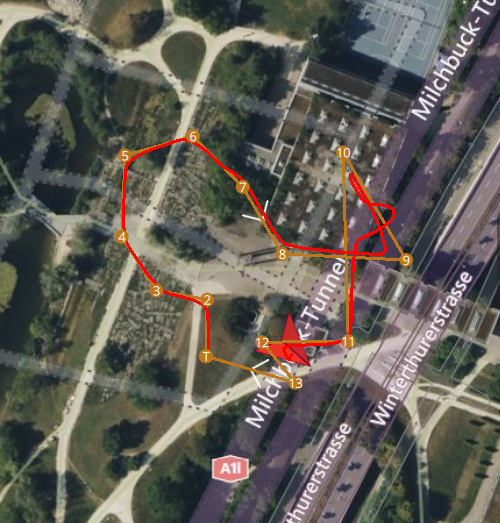
\includegraphics[width=0.5\textwidth]{files/images/path_soglia_fissa2 (1).png}
    \caption{Andamento del drone del test volo con guasto su potenza motore del 20\% su motore 2}
    \label{Risultato volo con guasto su potenza motore del 20\% su motore 2}
\end{figure}
\noindent

\begin{figure}[H]
    \centering
    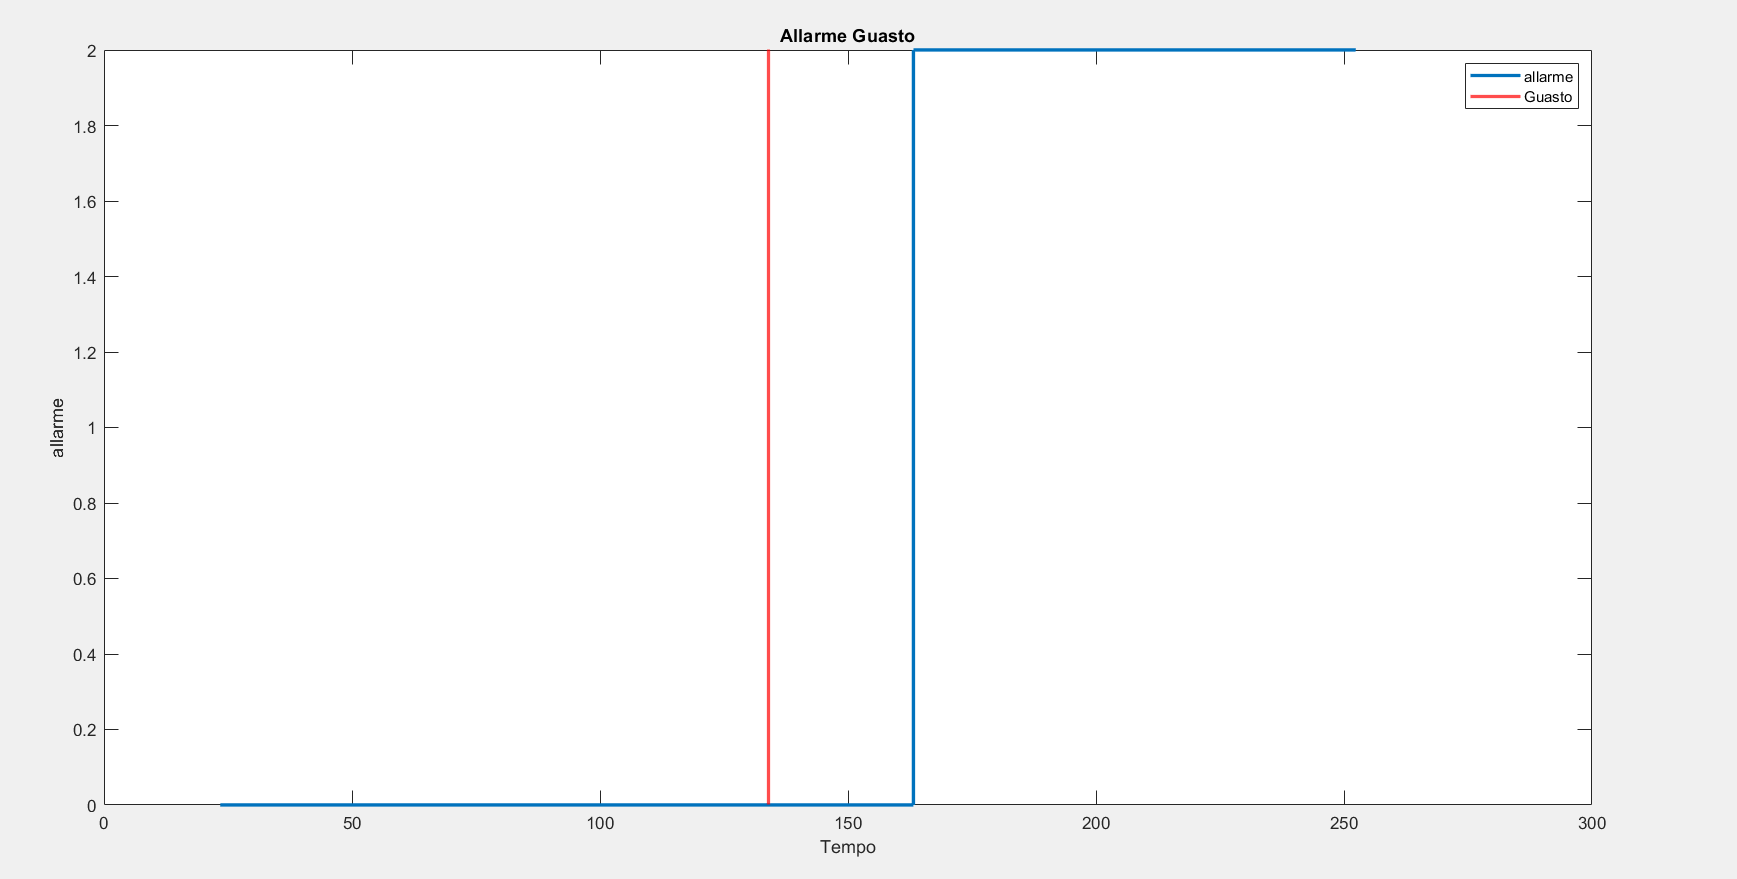
\includegraphics[width=\textwidth]{files/images/path_soglia_fissa2 (2).png}
    \caption{Allarmi del test volo con guasto su potenza motore del 20\% su motore 2}
    \label{Allarmi del test volo con guasto su potenza motore del 20\% su motore 2}
\end{figure}
\noindent

\begin{figure}[H]
    \centering
    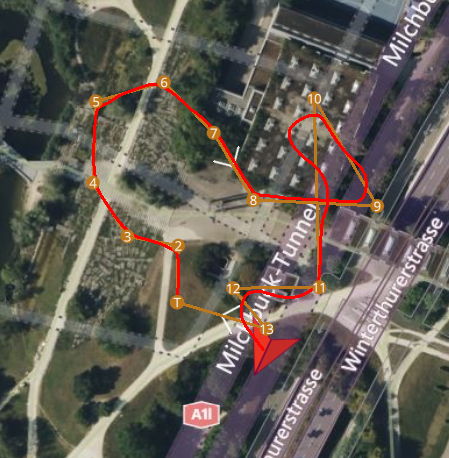
\includegraphics[width=0.5\textwidth]{files/images/path_soglia_fissa3 (2).png}
    \caption{Andamento del drone del test volo con guasto su potenza motore del 20\% su motore 3}
    \label{Risultato volo con guasto su potenza motore del 20\% su motore 3}
\end{figure}
\noindent

\begin{figure}[H]
    \centering
    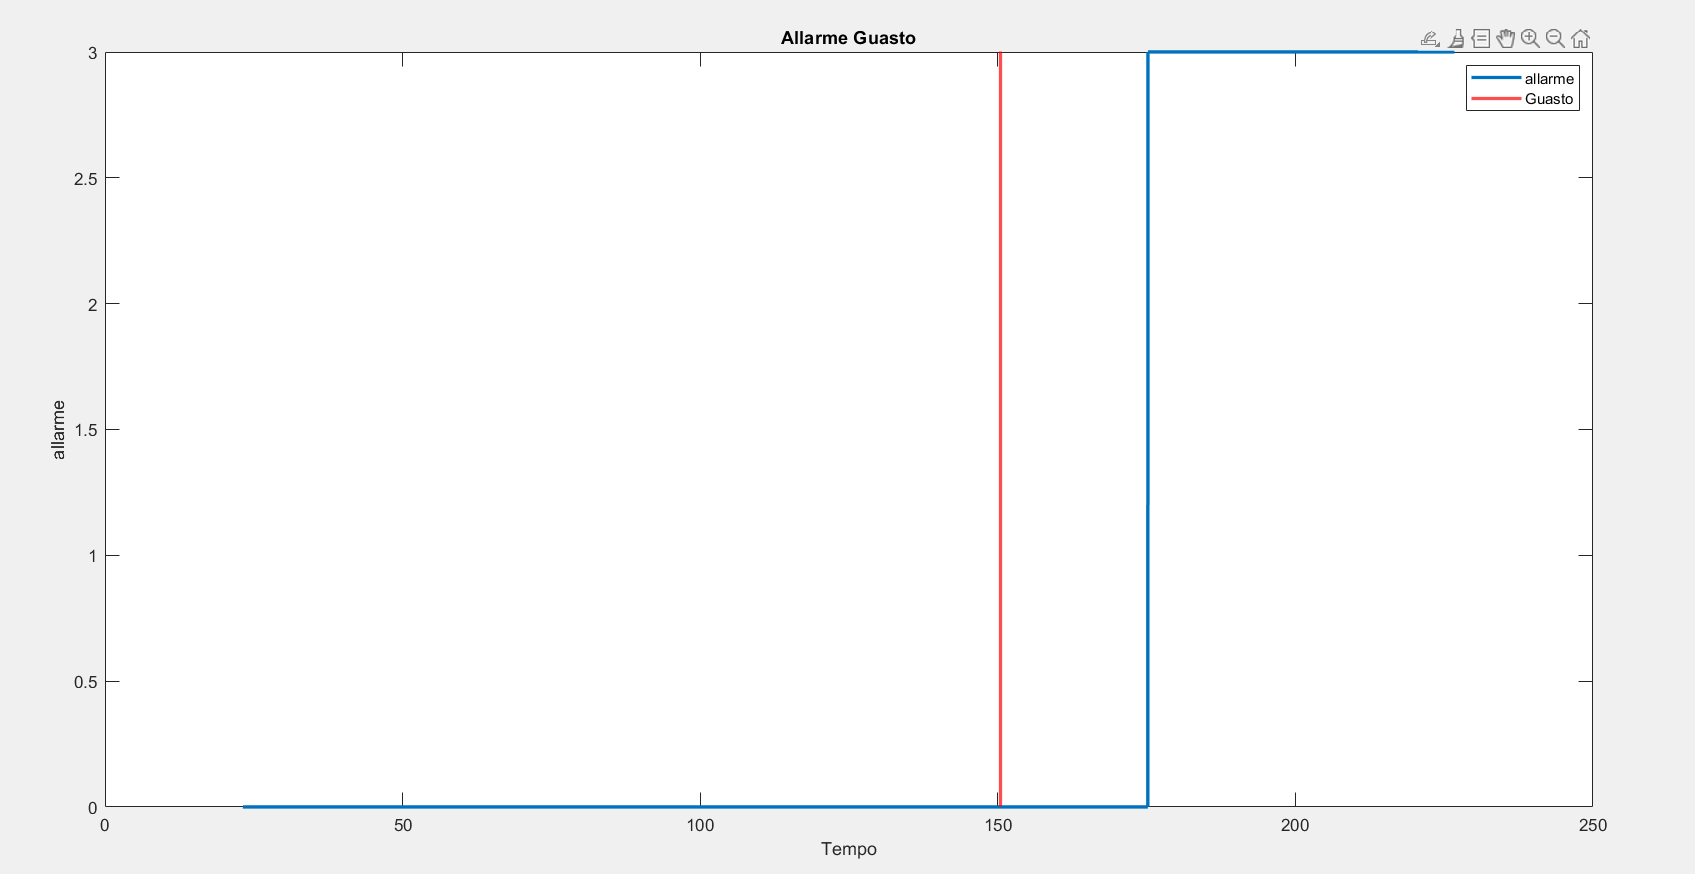
\includegraphics[width=\textwidth]{files/images/path_soglia_fissa3 (1).png}
    \caption{Allarmi del test volo con guasto su potenza motore del 20\% su motore 3}
    \label{Allarmi del test volo con guasto su potenza motore del 20\% su motore 3}
\end{figure}
\noindent

\begin{figure}[H]
    \centering
    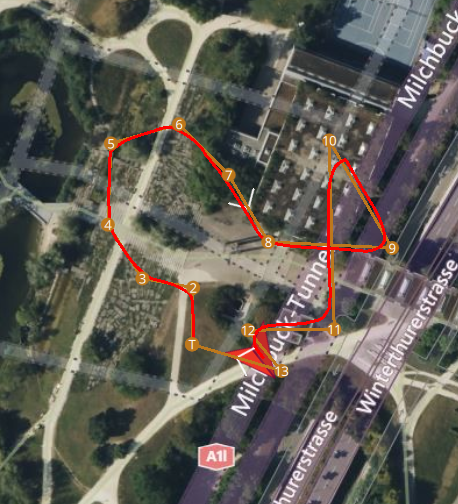
\includegraphics[width=0.5\textwidth]{files/images/path_soglia_fissa4 (2).png}
    \caption{Andamento del drone del test volo con guasto su potenza motore del 20\% su motore 4}
    \label{Risultato volo con guasto su potenza motore del 20\% su motore 4}
\end{figure}
\noindent

\begin{figure}[H]
    \centering
    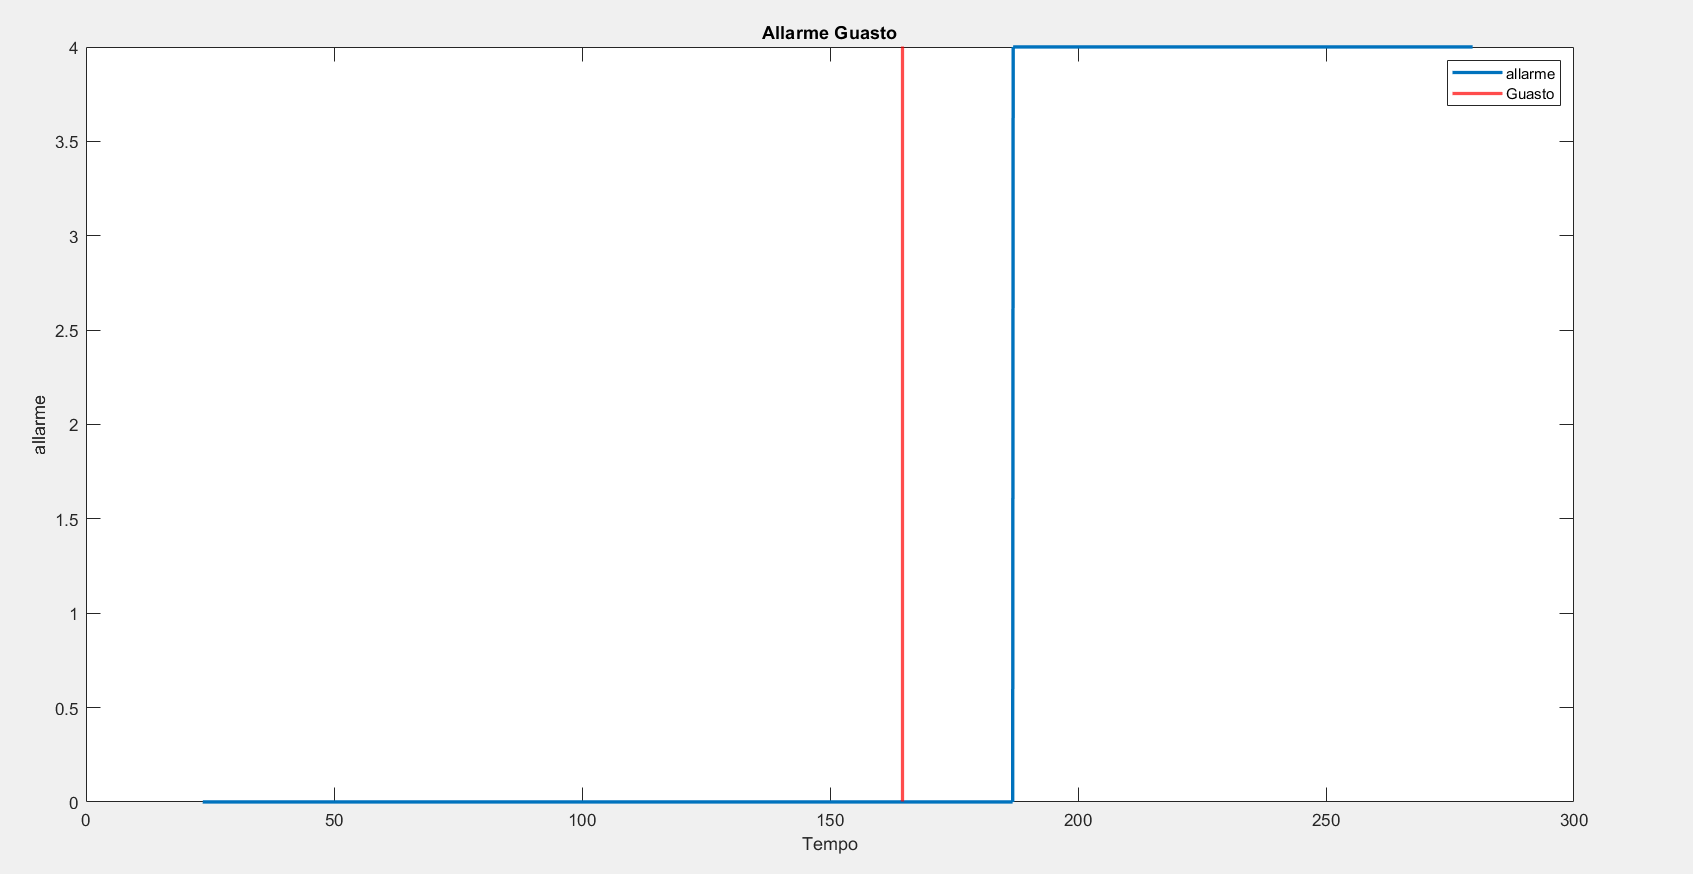
\includegraphics[width=\textwidth]{files/images/path_soglia_fissa4 (1).png}
    \caption{Allarmi del test volo con guasto su potenza motore del 20\% su motore 4}
    \label{Allarmi del test volo con guasto su potenza motore del 20\% su motore 4}
\end{figure}
\noindent

\section{Rilevamento dei Guasti con Soglia Adattiva}

Nella fase successiva del nostro studio, abbiamo esplorato un approccio di rilevamento dei guasti con soglia adattiva. Questo metodo si basa sull'utilizzo degli errori degli angoli di pitch e roll, analogamente alla sezione precedente.
\\
La soglia adattiva è stata calcolata nel seguente modo:
\begin{equation}
\text{PitchThreshold} = 0.1 + \left(\text{mean}(PitchBufferDes) \times \text{mean}(PitchBuffer)\right)
\end{equation}
\begin{equation}
\text{RollThreshold} = 0.1 + \left(\text{mean}(RollBufferDes) \times \text{mean}(RollBuffer)\right)
\end{equation}
\noindent
Queste equazioni rappresentano il calcolo delle soglie adattive per il rilevamento dei guasti, dove il valore di partenza 0.1 viene aggiunto a un contributo basato sul prodotto delle medie degli errori di pitch e roll e dei valori desiderati di pitch e roll.
\\
Per implementare il rilevamento dei guasti con soglia adattiva, abbiamo sviluppato un algoritmo che regola dinamicamente le soglie di rilevamento in base alla variazione del valore desiderato di angolo. La struttura blocchi all'interno di Quadcopter\_ControllerWithNavigation è simile a quello inserito per la soglia fissa (Fig. \ref{Rilevamento guasti con soglia adattiva Quadcopter\_ControllerWithNavigation}).
\\
\begin{figure}[H]
    \centering
    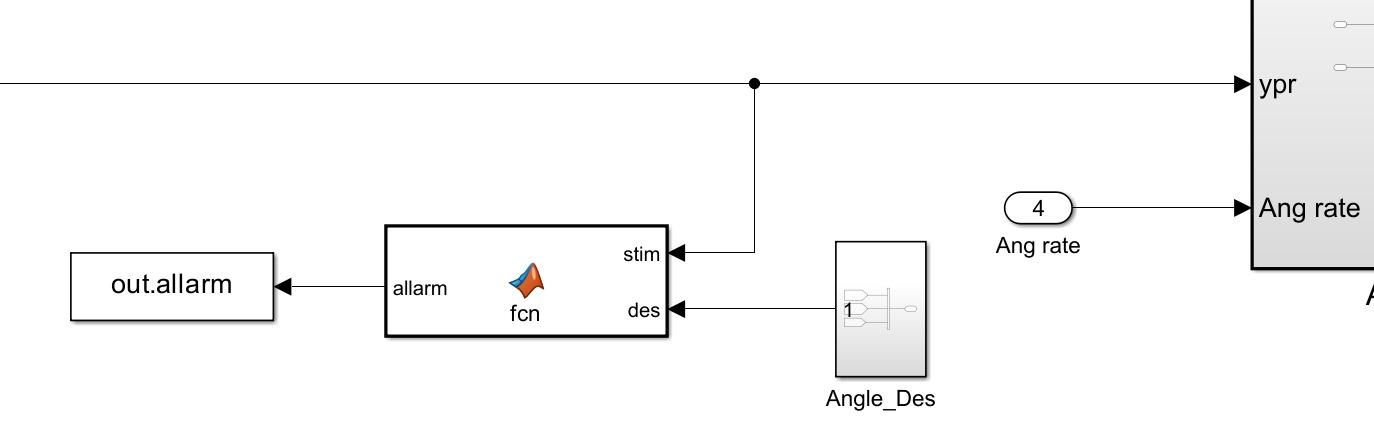
\includegraphics[width=0.5\textwidth]{files/images/WhatsApp Image 2024-03-15 at 18.28.16.jpeg}
    \caption{Rilevamento guasti con soglia adattiva Quadcopter\_ControllerWithNavigation}
    \label{Rilevamento guasti con soglia adattiva Quadcopter\_ControllerWithNavigation}
\end{figure}
\noindent
Il codice all'interno della MATLAB function è il seguente.
\begin{lstlisting}[language=Matlab, caption={Descrizione del codice}, label={lst:codice_matlab}]
function allarm = fcn(stim, des)
    persistent PitchBuffer RollBuffer 
    PitchBufferDes RollBufferDes
    if isempty(PitchBuffer)
        PitchBuffer = zeros(1, 500);
        RollBuffer = zeros(1, 500);
        PitchBufferDes = zeros(1, 500);
        RollBufferDes = zeros(1, 500);
    end

    % Calcolo gli errori di Pitch e Roll
    Pitch_Error = des(2) - stim(2);
    Roll_Error = des(3) - stim(3);

    % Per evitare che la media dia errore per i NaN, 
    sostituisco con 0
    if(isnan(Pitch_Error) && isnan(Roll_Error))
       Pitch_Error = 0;
       Roll_Error = 0;
    end

    % Aggiorna i buffer
    PitchBuffer = [PitchBuffer(2:end), Pitch_Error];
    RollBuffer = [RollBuffer(2:end), Roll_Error];
    PitchBufferDes = [PitchBufferDes(2:end), des(2)];
    RollBufferDes = [RollBufferDes(2:end), des(1)];;

    % Soglia Adattiva 
    PitchThreshold = 0.1 + 
    (mean(PitchBufferDes)*mean(PitchBuffer));
    RollThreshold = 0.1 + 
    (mean(RollBufferDes)*mean(RollBuffer));

    % Guasto Motore 1 del -20%
    if (mean(PitchBuffer) > PitchThreshold && 
    mean(RollBuffer) < -RollThreshold)
        allarm = 1;
    % Guasto Motore 2 del -20%
    elseif (mean(PitchBuffer) < -PitchThreshold && 
    mean(RollBuffer) > RollThreshold)
        allarm = 2;
    % Guasto Motore 3 del -20%
    elseif (mean(PitchBuffer) > PitchThreshold && 
    mean(RollBuffer) > RollThreshold)
        allarm = 3;
    % Guasto Motore 4 del -20%
    elseif (mean(PitchBuffer) < -PitchThreshold && 
    mean(RollBuffer) < -RollThreshold)
        allarm = 4;
    else
        allarm = 0;
    end
end
\end{lstlisting}
\noindent
Vengono inizializzati quattro buffer per registrare gli errori di pitch e roll, così come i valori desiderati di pitch e roll. Questi buffer vengono utilizzati per calcolare le medie degli errori nel tempo. Viene calcolato l'errore tra gli angoli desiderati e quelli stimati di pitch e roll. Gli errori di pitch e roll vengono aggiunti ai buffer e gli elementi più vecchi vengono rimossi per mantenere una dimensione fissa dei buffer. Le soglie adattive per il rilevamento dei guasti vengono calcolate in base alle medie degli errori di pitch e roll e dei valori desiderati di pitch e roll. Le soglie adattive si adattano dinamicamente alle variazioni nelle condizioni di volo. Viene eseguito il rilevamento dei guasti confrontando le medie degli errori di pitch e roll con le soglie adattive. Se le condizioni corrispondono a un guasto specifico, viene attivato l'allarme corrispondente al motore interessato.
\\
Durante la fase di volo, il nostro algoritmo monitora costantemente gli errori degli angoli di pitch e roll e aggiorna le soglie di rilevamento.
\\
\begin{figure}[H]
      \centering
      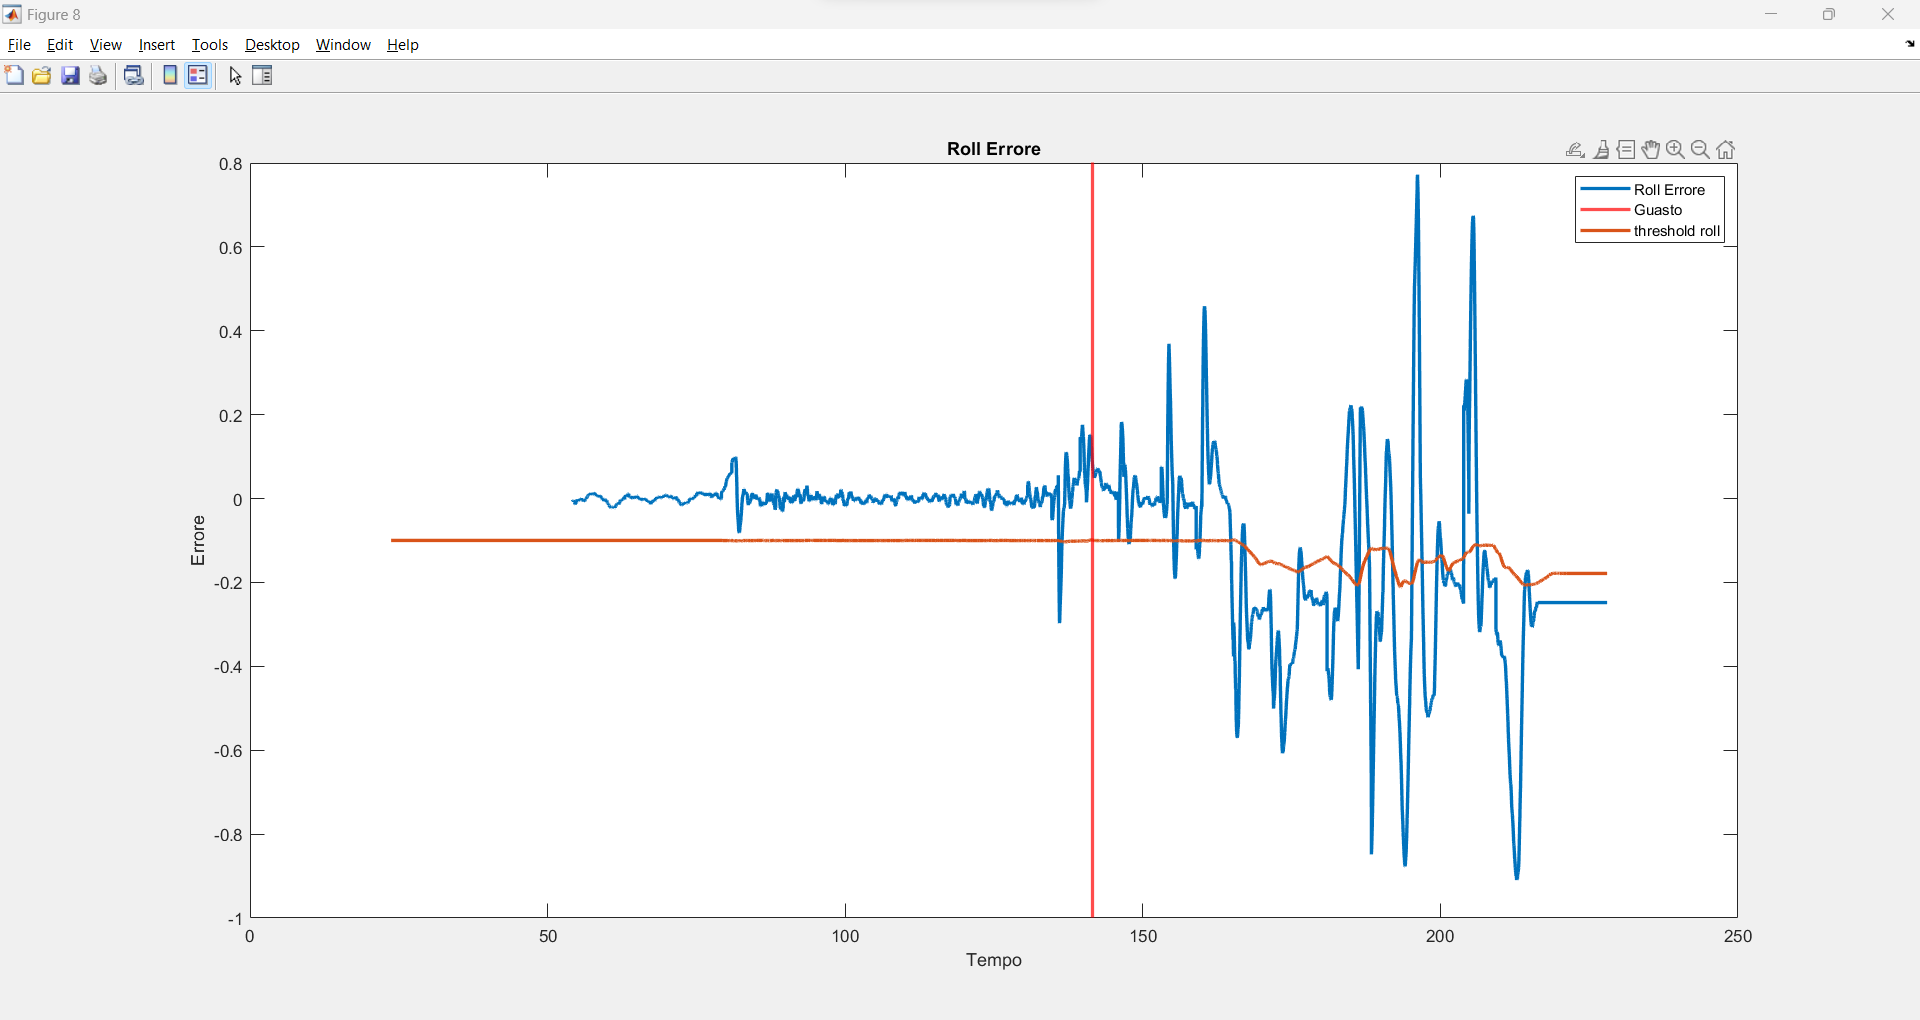
\includegraphics[width=\linewidth]{files/images/soglia_adattiva_roll.png} % Imposta la larghezza dell'immagine al 50% della larghezza del testo
      \caption{Soglia Adattiva Roll} % Didascalia sotto l'immagine
      \label{fig:Soglia adattiva Roll} % Etichetta per fare riferimento all'immagine nel testo
\end{figure}%
\begin{figure}[H] % Definisci la larghezza della seconda minipage (50% della larghezza della pagina)
        \centering
        \includegraphics[width=\linewidth]{files/images/soglia_adattiva_pitch.png} % Imposta la larghezza dell'immagine al 50% della larghezza del testo
        \caption{Soglia Adattiva Pitch} % Didascalia sotto l'immagine
      \label{fig:Soglia Adattiva Pitch} % Etichetta per fare riferimento 
\end{figure}
\begin{figure}[H]
    \centering
    \includegraphics[width=\textwidth]{files/images/allarmi_soglia_adattiva.png}
    \caption{Allarmi rilevati con soglia adattiva con perdita di potenza del 20\% sul motore 1}
    \label{Allarmi soglia adattiva}
\end{figure}
\noindent
I risultati preliminari ottenuti utilizzando il rilevamento dei guasti con soglia adattiva sono simili a quelli con soglia fissa con buffer (Fig. \ref{Allarmi soglia adattiva}). Abbiamo osservato che il guasto viene rilevato dopo una prima curva che il drone effettua.
\\
Ulteriori studi e test sono necessari per valutare completamente le prestazioni e l'efficacia del rilevamento dei guasti con soglia adattiva, ma i risultati preliminari indicano un potenziale significativo per il rilevamento guasti sui motori.
 \clearemptydoublepage
\chapter{Conclusioni} \clearemptydoublepage
\include{UserManual} \clearemptydoublepage
%\addcontentsline{toc}{chapter}{Elenco delle figure}%


%possibilità di poter riusare le cit per qualsiasi progetto latex
\nocite{*}


\clearemptydoublepage

\addcontentsline{toc}{chapter}{Bibliography}
\nocite{*}
\bibliographystyle{plain}
\bibliography{files/frontbackmatters/bibliography}

\listoffigures


\end{document}
